% ============================================================================
%  Strictly Online Reinforcement Learning in Recurrent Spiking Neural Networks
%  Without Structured Gradient Feedback  (method: "distributed e-prop")
%
%  INITIAL PAPER DRAFT (two-column). Built from the master's thesis
%  "Distributed E-prop and TD(lambda)".
%
%  NOTES FOR THE AUTHOR
%  --------------------
%  * Class: generic twocolumn article + natbib (author-year), chosen because it
%    preserves your \citep/\citet, \eqref, [H] floats and booktabs tables.
%    To target a venue, swap the first line for e.g. \documentclass{IEEEtran}
%    (numbered cites, use \cite), the NeurIPS style file, or a journal class.
%  * Wide multi-panel figures use figure* to span both columns; portrait/2-panel
%    ones use a single column. Adjust per your final figure aspect ratios.
%  * All \includegraphics paths point at the real thesis figure filenames under
%    images/. \graphicspath includes images/ and figures/.
%  * Bibliography: project references.bib via \bibliography{references}.
%  * Anywhere a specific number/figure is cited it comes from Chapter 4 of the
%    thesis; double-check against your final figures before submission.
% ============================================================================

% -- TEXT SIZE: article supports 10/11/12pt only. For 9pt/9.5pt, swap
%    "article" for "extarticle" below and set [9pt,twocolumn] (identical
%    otherwise). Keep it here so the whole document rescales from one place.
\documentclass[10pt,twocolumn]{article}

% -- MARGINS / DENSITY: tighter than article's defaults so the two columns
%    carry more text. Loosen margin= to 1in, or widen columnsep, to taste.
\usepackage[letterpaper,margin=0.5in,bottom=0.9in,footskip=0.4in,columnsep=0.2in]{geometry}

\usepackage{fontspec}
\setmainfont{Latin Modern Roman}   % keeps your current serif body font
\setsansfont{Fira Sans}[UprightFont=*-Light, BoldFont=*-Regular]
\setsansfont{Fira Sans}[LetterSpace=2.0]
\setsansfont{IBM Plex Sans}
\usepackage{amsmath,amssymb,amsfonts}
\IfFileExists{bbm.sty}{\usepackage{bbm}}{\providecommand{\mathbbm}[1]{\mathbf{##1}}} % \mathbbm{1} (bbm if available, else bold fallback)
\usepackage{graphicx}
\usepackage{float}               % [H]
\usepackage{booktabs}            % \toprule etc.
\usepackage{array}
\usepackage{siunitx}
\usepackage[hidelinks]{hyperref}
\usepackage{url}
\usepackage[round]{natbib}       % author-year; -> \citep, \citet
\usepackage{authblk}
\usepackage{caption}
\usepackage{sectsty}          % sans-serif headings (numbered), serif body
\sectionfont{\sffamily}
\subsectionfont{\sffamily\normalsize}
\captionsetup{font=small,labelfont={sf,bf}}

\graphicspath{{images/}{figures/}}

\usepackage{fancyhdr}
\pagestyle{fancy}
\fancyhf{}
\fancyfoot[L]{\sffamily\footnotesize Strictly Online RL in RSNNs with Distributed E-prop}
\fancyfoot[R]{\sffamily\small\thepage}
\renewcommand{\headrulewidth}{0pt}
\renewcommand{\footrulewidth}{0.4pt}

\fancypagestyle{plain}{%
  \fancyhf{}
\fancyfoot[L]{\sffamily\footnotesize Strictly Online RL in RSNNs with Distributed E-prop}
\fancyfoot[R]{\sffamily\small\thepage}
  \fancyfoot[R]{\sffamily\small\thepage}
  \renewcommand{\headrulewidth}{0pt}
  \renewcommand{\footrulewidth}{0.4pt}
}

\AtBeginDocument{\thispagestyle{empty}}  % suppress header+footer on page 1

\usepackage{algorithm}
\usepackage{algpseudocode}

\usepackage{xcolor}
\newcommand{\pending}[1]{\textcolor{red}{\bfseries[PENDING RERUN#1]}}
\newcommand{\todo}[1]{\textcolor{red}{\bfseries[TODO: #1]}}
\newcommand{\tbd}{\textcolor{red}{\bfseries ?}} % table cell still to be filled

\newcommand{\variant}[1]{\textsf{#1}} % variant tags, as named in figure legends

% -- FLOAT PLACEMENT: let full-width (figure*) floats take more of a page so
%    they do not queue up and drift past the text that references them.
\setcounter{dbltopnumber}{3}
\renewcommand{\dbltopfraction}{0.9}
\renewcommand{\dblfloatpagefraction}{0.8}
\renewcommand{\topfraction}{0.9}
\renewcommand{\textfraction}{0.07}
\renewcommand{\floatpagefraction}{0.8}

% ---------------------------------------------------------------------------
\title{\sffamily\bfseries Strictly Online Reinforcement Learning in Recurrent Spiking
Neural Networks Without Structured Gradient Feedback\thanks{Code and experiments: \url{https://github.com/Nordest27/ml_genn}.}}

\author[1]{Edgar Sarria Tenes}
\affil[1]{Affiliation \\ \texttt{edgar.sarria@estudiantat.upc.edu}}
\date{}

% ---------------------------------------------------------------------------
\begin{document}
\maketitle

\begin{abstract}
Biological brains learn continuously from a single stream of experience, in
real time and under tight energy budgets, without replaying stored data or
pausing at episode boundaries, a mode of learning whose lifelong adaptivity and
efficiency machine learning has yet to match. Reinforcement learning in spiking
recurrent neural networks (SRNNs) is a natural but demanding setting in which to
pursue it: reward is delayed and sparse, spikes are non-differentiable, and
credit must be assigned across long delays. We study the \emph{strictly online},
\emph{continuing} version of this problem: learning forward in time from
quantities that are local in both space and time, updating at every timestep,
with no replay, no stored trajectories, and no resets at episode boundaries.
These constraints rule out most learning rules for recurrent networks. E-prop,
which factorises the gradient into a local eligibility trace and a per-neuron
learning signal, is among the few that remain applicable and, we argue, the most
promising; even e-prop, however, must route its learning signal to each neuron
through structured feedback weights. We ask whether that structure is needed
at all, and introduce \emph{distributed e-prop}, a family of fully local rules
in which a single temporal-difference error is broadcast and each neuron acts
as a stochastic actor, perturbing its own membrane potential and correlating a
filtered trace of that perturbation with the shared scalar, gated by the e-prop
pseudo-derivative. Surprisingly, this much poorer signal is enough: on Snake,
the strongest variant learns faster than adaptive-feedback e-prop, reaches a
higher reward rate, and learns a more accurate critic, and the pseudo-derivative
gate proves essential.\pending{: Pac-Man and Tic-Tac-Toe results to be added.}
\end{abstract}

% ===========================================================================
\section{Introduction}
\label{sec:intro}

Continuous control, real-time sensing, and embodied agents are among the
settings where recurrent networks would be most useful, and they all share a
structure that standard recurrent training does not fit. In each of them,
data arrives as an uninterrupted stream, decisions must be made immediately
as that stream unfolds, and there is no natural point at which the system can
pause and compute gradients before continuing. The dominant recipe for
training recurrent networks assumes the opposite of all three: it assumes a
sequence with a beginning and an end, the freedom to wait until that end is
reached, and enough memory to hold the whole sequence in the meantime. Backpropagation through time (BPTT)~\citep{Werbos1990BackpropagationTT}
makes this assumption explicit: it stores the full history of network activity
as the sequence plays out, and only once the sequence ends does it replay that
history backward to compute a gradient. As interaction continues indefinitely,
so does the history BPTT must store, so its memory grows without bound and its
updates are delayed until the sequence stops, an event that a continuous
stream never provides. Truncating the window over which gradients are
computed (TBPTT)~\citep{WilliamsZipser1995} fixes the memory problem by
capping how much history is kept, but that same cap now limits how far back
in time credit can be assigned, so long-range dependencies that fall outside
the window are simply invisible to learning. The alternative is to compute the
gradient forward in time instead of backward: real-time recurrent learning
(RTRL)~\citep{RTRL} does exactly this, propagating an exact influence matrix
forward as the network runs, so that a gradient is always available without
ever needing to stop and look back. RTRL is local in time but not in space:
its influence matrix holds the sensitivity of every unit's state to every
parameter, so updating any single weight requires information from the whole
network. That exactness also has a steep price: for $n$ fully connected units
the influence matrix has $O(n^3)$ entries and costs $O(n^4)$ operations to
update every step, which puts RTRL out of reach for anything beyond small
networks. BPTT and RTRL therefore sit at opposite ends of the same tradeoff,
unbounded memory against prohibitive, spatially non-local compute, and it is this gap
between them that forward-in-time, local approximations of the recurrent
gradient are built to close.

Reinforcement learning compounds the difficulty: the only learning signal is a
scalar reward that may arrive long after the activity that produced it, so
temporal credit must be assigned across long delays. Standard RL typically
meets this by storing experience in a replay buffer, treating past
trajectories as a dataset that can be sampled and reused long after they were
collected. Even methods that skip replay still need the trajectory to be
collected in full before learning can happen, since backpropagating through
time requires the whole sequence to already exist before a gradient can be
computed by running backward through it. A strictly online setting rules out
both: there is no buffer to sample from and no completed trajectory to
backpropagate through, so credit must be assigned as the stream unfolds, in
real time.

We call this setting \emph{strictly online}: the agent learns from a single,
uninterrupted stream of experience, using only quantities that are local in
both space and time, with no replay buffer. The only memory it can draw on for
learning is the network's own activity together with its eligibility traces,
so credit flows forward in real time, never through a backward pass. This
online gradient can in principle be applied on any schedule, every step, every
action window, or every episode, since accumulating it is not itself a form of
stored history. We do not rule out the coarser schedules on principle; some
form of online accumulation may well be compatible with a strictly online
agent. What we lack is a general, task-agnostic rule for choosing the window:
accumulating over an action window or an episode requires knowing, in advance
and per task, where the boundaries of ``enough evidence'' fall, and supplying
that boundary from outside is itself a form of timing handed to the learning
rule, not discovered by it. Absent such a rule, we adopt the one
schedule that needs no external tuning at all and update every single
timestep throughout, the most conservative default and the one most faithful
to a continuously learning, clock-free agent. This is a stronger requirement
than the ``online'' label usually carries, where methods still lean on stored
roll-outs. We do not aim for full biological plausibility; we keep the
constraints that are most consequential for online learning, the same
constraints that govern learning on neuromorphic hardware.

We have not yet removed every piece of task-specific timing. The policy head
samples a discrete action from a softmax at fixed action windows of $K=30$
integration steps, so the policy-gradient term of the learning signal is
delivered only at those sampling steps; in distributed e-prop this term
reaches only the output weights, since the hidden weights see only the
broadcast TD error. The action window is therefore an externally supplied
clock, the same kind of outside timing we argued above should not be handed
to the update schedule. Letting the learning rule, rather than the task
configuration, handle action timing is an open problem, and making the agent
as task-agnostic as possible is the main direction for future work
(Section~\ref{sec:discussion}).

We pair this with a \emph{continuing}, non-episodic task formulation: the
network's internal state (membrane potentials, adaptation, and eligibility
traces) is never reset at game boundaries. This is a deliberate modelling
choice. Real embodied learning has no episode boundaries; forcing a reset
supplies an explicit boundary and wipes the network's state, handing the agent
a clean slate it would never have in a continuous stream. Keeping the state
continuous puts the burden of segmenting the stream and carrying credit across
it where it belongs: on the learning rule. Every result in this paper is
obtained under both constraints.

Together, these constraints leave very few learning rules standing. BPTT and
its truncated form need stored history and a backward pass; replay-based and
roll-out-based reinforcement learning need stored experience; RTRL is exact
but non-local in space, and its cost rules it out beyond small networks; and many of its cheaper
approximations rely on non-local operations or have not been shown to learn
reinforcement tasks from a single continuing stream. Of the forward-in-time,
local rules, e-prop is the most developed and has already been demonstrated
for reward-based learning in spiking networks, so we take it as the reference
for what current learning rules can achieve in this setting. Rules of this kind
have a further advantage over BPTT and RTRL, which the rule we introduce shares
rather than adds: they never multiply derivatives along a path through time or
the network, so the magnitude of their updates cannot vanish or explode with
path length or delay (Section~\ref{sec:distributed}).

Spiking recurrent networks (SRNNs) are an attractive substrate for this
regime: they integrate information through their own dynamics, communicate
through sparse discrete events, and map naturally onto low-power neuromorphic
hardware \citep{Davies2018Loihi,Painkras2013SpiNNaker}. E-prop
\citep{eprop2020}, a forward-in-time approximation of RTRL, makes online
training of SRNNs tractable by factorising the loss gradient into a
neuron-local \emph{eligibility trace}, computed purely forward in time, and a
neuron-specific \emph{learning signal} $L^t_j$ that approximates
$\mathrm{d}E/\mathrm{d}z^t_j$. In the reinforcement-learning form, an
actor--critic head produces $L^t_j$ and routes it back to each hidden neuron
through structured feedback weights.

That feedback projection is where e-prop pays for its locality. The learning
signal only approximates the true gradient, and the approximation quality
depends on the feedback scheme. \emph{Symmetric} weights (tied to the forward
readout) give any neuron not directly connected to an output head no signal at
all, so learning fails outright once the causal path length exceeds one.
\emph{Random} and \emph{adaptive} feedback reach all neurons but still
accumulate approximation error with depth. This motivates our central
question: \emph{is structured feedback necessary at all, or can a network
learn if each neuron receives only a single global scalar?}

We answer it with \textbf{distributed e-prop}. Drawing on the connection
between perturbation learning and policy gradients
\citep{fiete2006gradient,salimans2017evolutionstrategiesscalablealternative},
we treat each neuron as an independent stochastic actor with a Gaussian policy
over its own membrane potential. Each neuron draws a small perturbation, keeps
a filtered trace of it, and, when the broadcast temporal-difference error
$\delta_t$ arrives, correlates that trace with $\delta_t$ to update its
incoming weights. No feedback weights exist and no policy gradient is routed;
the global agent policy \emph{emerges} from the collective behaviour of many
local actors optimising against the same shared scalar. This is the
philosophy of evolution strategies: \emph{was the outcome better or worse
than expected, and what did I try?}, run here online, in continuous time,
inside a single recurrent trajectory. Concretely, each neuron $j$ draws a
membrane perturbation
$\varepsilon_j^t$, keeps a filtered trace
$\xi_j^t = \alpha\,\xi_j^{t-1} + \varepsilon_j^t$ of it, and updates each incoming
synapse by
\begin{equation}
\Delta W_{ji} \;\propto\; \sum_t \delta_t\;
\mathcal{F}_{\lambda}\!\left(
\frac{(1-\alpha^2)}{\sigma_j^2}\,\xi_j^t\, e_{ji}^t \right),
\label{eq:intro-update}
\end{equation}
where $\delta_t$ is the broadcast TD error, $e_{ji}^t$ the e-prop eligibility
trace, $\sigma_j^2$ the exploration variance, $\alpha$ the membrane decay, and
$\mathcal{F}_{\lambda}$ a low-pass filter. Only $\delta_t$ is non-local; no
feedback matrix appears anywhere in Eq.~\eqref{eq:intro-update}.
Section~\ref{sec:distributed} derives this rule and its variants.

One might expect such an impoverished signal to give, at best, a weaker
alternative to e-prop's structured feedback. Instead, in this strict setting,
its strongest variant matches or exceeds the best e-prop variant we tested: on
Snake it learns faster, reaches a higher reward rate, and learns a more
accurate critic than adaptive-feedback e-prop
(Section~\ref{sec:results-snake}).\pending{: extend to Pac-Man and
Tic-Tac-Toe.}

This paper makes three main contributions. \textbf{(i)}~We evaluate
reward-based learning in SRNNs under a strictly online, continuing protocol, a
setting in which few existing learning rules apply, taking e-prop with
symmetric and adaptive feedback as the most promising existing candidates and
comparing them against an activity-matched, reservoir-computing-inspired
baseline whose recurrent weights receive no task-driven learning
(Section~\ref{sec:results}). \textbf{(ii)}~We introduce \emph{distributed
e-prop} (Section~\ref{sec:distributed}), a family of fully local, online
learning rules for reward-based training of SRNNs that use no structured
gradient feedback, with variants that inject noise at the neuron or the
synapse; as supporting machinery, we also give a decoupled TD($\lambda$)
formulation (Section~\ref{sec:tdlambda}) that keeps a short-horizon critic
stable in the continuing setting while preserving long-range credit. We find
the e-prop pseudo-derivative, reused as a gate, to be essential: without it
the rule fails (Section~\ref{sec:results-snake}). \textbf{(iii)}~We show that,
in this setting, the strongest variant matches or exceeds adaptive-feedback
e-prop: it learns faster, reaches a higher reward rate, and learns a critic
that tracks the realised return more closely
(Section~\ref{sec:results-snake}).\pending{: extend to Pac-Man and
Tic-Tac-Toe.}

% ===========================================================================

\section{Related Work}
\label{sec:related}

\paragraph{Online learning in recurrent networks.}
The exact recurrent gradient is given by BPTT~\citep{Werbos1990BackpropagationTT},
whose memory grows with sequence length; truncation (TBPTT) bounds this at the
cost of the credit horizon~\citep{WilliamsZipser1995}, and vanishing gradients
further limit how far credit can travel~\citep{learningLongTermHard}. RTRL
computes the gradient forward in time~\citep{RTRL}, but it is non-local in
space, tracking the sensitivity of every unit to every parameter at $O(n^3)$
storage and $O(n^4)$ compute per step,
motivating cheaper forward approximations: UORO gives an unbiased low-rank
estimator~\citep{UORO}, OSTL separates spatial and temporal credit for deep
spiking networks~\citep{OSTL}, and synthetic gradients decouple modules through
predicted feedback~\citep{Jaderberg2016}. E-prop~\citep{eprop2020} is the member
of this family we build on, factorising the gradient into a forward,
synapse-local eligibility trace and a per-neuron learning signal; the rate-based
RFLO rule is a close analogue~\citep{murray2019local}. Among these methods,
e-prop is, to our knowledge, the most developed for reward-based learning in
spiking networks under forward, local constraints, which is why we use it as
the reference for the strict setting studied here. Distributed e-prop stays
within this forward, local regime but removes the structured learning signal.

\paragraph{Credit assignment without symmetric feedback.}
Backpropagation requires symmetric feedback weights, which feedback alignment
showed to be unnecessary: fixed random feedback can still carry a usable error
signal~\citep{Lillicrap2016}, a principle extended to recurrent networks in
RFLO~\citep{murray2019local} and available in e-prop as its random and adaptive
feedback variants~\citep{eprop2020}. A more radical step drops backpropagated
feedback in favour of locally computed TD errors: \citet{guan2024artificialdopamine}
recently showed that per-layer TD errors, each computed locally and
distributed synchronously within its layer, closer to how dopamine is actually
delivered, may be sufficient to learn complex RL tasks in non-spiking deep
Q-networks. Distributed e-prop goes further for spiking recurrent networks: it
uses no feedback matrix of any kind and a single broadcast scalar, the global
TD error, together with each neuron's local perturbation and eligibility
traces.

\paragraph{Perturbation-based and reward-modulated learning.}
Correlating stochastic perturbations with a global reward has a long history,
from stochastic error-descent~\citep{Cauwenberghs1992} and
REINFORCE~\citep{Williams1992REINFORCE} to conductance perturbation in spiking
neurons~\citep{fiete2006gradient} and modern evolution
strategies~\citep{salimans2017evolutionstrategiesscalablealternative}. In
neuroscience the same ingredients recur as three-factor, reward-modulated STDP,
where a global neuromodulator gates a local Hebbian trace
\citep{Fremaux2016NeuromodulatedSTDP,Izhikevich2007DistalReward,Florian2007RewardSTDP,Legenstein2008RewardSTDP},
and as continuous-time actor-critic learning in spiking
networks~\citep{Frmaux2013ReinforcementLU}. Our rule sits at this intersection:
a perturbation-based policy gradient whose variance is tamed by the e-prop
eligibility trace and its surrogate derivative~\citep{Neftci2019Surrogate}, run
online and in continuous time. It is complementary to value-based spiking RL
such as spiking Q-learning~\citep{Chen2022SpikingQLearning}.

% ===========================================================================
\section{Background}
\label{sec:background}

\paragraph{E-prop.}
We use adaptive leaky integrate-and-fire (ALIF) neurons. For a recurrent weight
$W_{ji}$, e-prop factorises the gradient as
\begin{equation}
\frac{\mathrm{d}E}{\mathrm{d}W_{ji}} = \sum_t L^t_j\,\bar{e}^{\,t}_{ji},
\qquad L^t_j \approx \frac{\mathrm{d}E}{\mathrm{d}z^t_j},
\label{eq:eprop-factorisation}
\end{equation}
where $\bar e^{\,t}_{ji}$ is a filtered eligibility trace built from local,
forward-in-time quantities and $L^t_j$ is the only signal that must reach
neuron $j$. The eligibility trace $e^t_{ji}=\psi^t_j(\bar z^t_i-\beta\,
\epsilon^{t-1}_{ji})$ combines the low-pass-filtered presynaptic spike train
$\bar z^t_i$ with the \emph{pseudo-derivative} $\psi^t_j$, a surrogate for the
non-differentiable spike threshold that is largest when the membrane is near
threshold.

\paragraph{Reward-based e-prop.}
For reinforcement learning, an actor--critic head~\citep{Konda2000ActorCritic} supplies $L^t_j$. Actions are
drawn from a softmax policy over the readout $y^t_k$; the critic yields the
TD error
\begin{equation}
\delta_t = R_{t+1} + \gamma\, V_{t+1} - V_t,
\label{eq:tderror}
\end{equation}
and the learning signal combines value and policy feedback,
\begin{equation}
L^t_j = -c_V B^V_j + \sum_k B^\pi_{kj}\!\left(\pi^t_k - \mathbbm{1}_{a_t=k}\right),
\label{eq:learning-signal}
\end{equation}
with feedback weights $B^V_j$, $B^\pi_{kj}$. The online update is
$\Delta W_{ji} = -\eta\sum_t \delta_t\,\mathcal{F}_{\gamma}(L^t_j\,\bar
e^{\,t}_{ji})$, where $\mathcal{F}_{\gamma}$ is a leaky filter. The feedback
matrices $B$ can be \emph{symmetric} (tied to the readout), \emph{random}, or
\emph{adaptive} (learned); all three provide each neuron a per-neuron
approximation of the gradient, and it is this projection that distributed
e-prop removes.

\paragraph{Perturbation learning and three-factor rules.}
A different tradition abandons structural credit accounting altogether:
perturb candidate parameters, observe the global outcome, and reinforce
perturbations that coincided with improvement
\citep{salimans2017evolutionstrategiesscalablealternative}. For spiking
neurons, node/conductance perturbation yields a REINFORCE-like estimator
directly from injected noise \citep{fiete2006gradient}. Such rules are
biologically evocative: they reduce to a global evaluative signal gating a
local activity trace, the structure of neuromodulated three-factor plasticity
\citep{Fremaux2016NeuromodulatedSTDP,Izhikevich2007DistalReward,
Florian2007RewardSTDP}. Their well-known weakness is variance that grows with
the number of perturbed parameters. Distributed e-prop inherits this lineage
and adds the e-prop eligibility gate, which we find essential for making it
work online, as described next.

% ===========================================================================
\section{Method}
\label{sec:method}

\subsection{A Decoupled TD($\lambda$) Update}
\label{sec:tdlambda}

One piece of supporting machinery is needed before the rules themselves. In the
standard TD($\lambda$) update the credit trace decays at $\gamma\lambda$, so a
single $\gamma$ both discounts the bootstrap target (Eq.~\eqref{eq:tderror}) and
bounds how far back a reward-prediction error is assigned. In the continuing,
non-episodic setting these roles conflict: with no terminal state and a noisy
spike-based critic, $\gamma$ must be small for the value estimate to stay
learnable, but a small $\gamma$ then caps the actor's credit horizon at
$\gamma\lambda\le\gamma$, sometimes below a single action. We therefore decouple
the two, dropping $\gamma$ from the actor and hidden-weight traces so that
$\lambda$ alone sets the horizon,
\begin{equation}
p^{\,t}_{ji} = \lambda\, p^{\,t-1}_{ji} + L^t_j\,\bar e^{\,t}_{ji},
\qquad \Delta W_{ji} = -\eta\sum_t \delta_t\, p^{\,t}_{ji},
\label{eq:actor-modified}
\end{equation}
while the critic keeps $\gamma$ (equivalently, runs at $\lambda_V=1$),
\begin{equation}
\nu^{\,t}_{ji} = \gamma\,\nu^{\,t-1}_{ji} + \bar e^{\,V,t}_{ji},
\qquad \Delta W^V_{ji} = \eta_V\sum_t \delta_t\,\nu^{\,t}_{ji}.
\label{eq:critic-modified}
\end{equation}
Reinstating $\gamma$ in Eq.~\eqref{eq:actor-modified} recovers standard
TD($\lambda$)~\citep{SuttonBarto2018}; dropping it is a deliberate, biased choice that preserves the
long-range credit a short $\gamma$ trace would suppress. Because each action
spans $K$ integration steps, per-step decays are
$\gamma_{\mathrm{step}}=\gamma^{1/K}$ and
$\lambda_{\mathrm{step}}=\lambda^{1/K}$; we use $\gamma=0.5$, $\lambda=0.8$
at the action level throughout.

\subsection{Distributed E-prop}
\label{sec:distributed}

\paragraph{Neurons as stochastic actors.}
Each neuron treats its own membrane potential as a continuous action drawn from
a Gaussian policy: at every step neuron $j$ samples
$v^t_j\sim\mathcal{N}(\mu^t_j,\sigma_j^2)$, centred on the value $\mu^t_j$ its
deterministic dynamics would have produced, with per-neuron exploration variance
$\sigma_j^2$. The sampled membrane $v^t_j$ is the action; the deviation
$\varepsilon^t_j = v^t_j-\mu^t_j\sim\mathcal{N}(0,\sigma_j^2)$ is the exploration
noise that drives the policy gradient (it is the score
$\nabla_{\mu^t_j}\log\pi = \varepsilon^t_j/\sigma_j^2$). Spikes are a
deterministic function of the sampled membrane,
$z^t_j=H(v^t_j-v_{\mathrm{th}})$, so this exploration reaches behaviour only
through the spike timing it produces. Because the membrane integrates over time,
the influence of past deviations decays through the membrane at it's same decay rate, so each neuron keeps a filtered \emph{perturbation trace}
\begin{equation}
\xi^t_j = \alpha\,\xi^{t-1}_j + \varepsilon^t_j,
\label{eq:perturbation-trace}
\end{equation}
its local memory of the activity that cannot be accounted by the deterministic dynamics.

\paragraph{The update rule.}
The exact likelihood-ratio (REINFORCE) estimator for this stochastic neuron
pairs each fresh perturbation with the input it modulated. Conditioning on the
previous sampled membrane, the score of step $t$ is $\varepsilon^t_j/\sigma_j^2$
and $\partial\mu^t_j/\partial W_{ji}=z^{t-1}_i$, giving
$\sum_t\varepsilon^t_j z^{t-1}_i/\sigma_j^2$. Each perturbation is scored once,
at the step it was injected; its lasting effect on the membrane, and through it
on later spikes and rewards, is credited only statistically, through its
correlation with the subsequent return. This principle is not new: correlating
injected noise with reward is the REINFORCE principle for stochastic
units~\citep{Williams1992REINFORCE}, and it has been applied to spiking neurons
both by perturbing conductances and correlating the perturbation with
presynaptic activity~\citep{fiete2006gradient} and by deriving policy-gradient
rules for stochastic spiking neurons~\citep{Florian2007RewardSTDP}.

We instead use the known membrane dynamics to credit that lasting effect
explicitly. Because the membrane is linear with known decay $\alpha$, the part
of $v^t_j$ that the deterministic dynamics do not account for is exactly the
perturbation trace $\xi^t_j$ of Eq.~\eqref{eq:perturbation-trace} (exactly so
between resets), and it is $\xi^t_j$, not the latest $\varepsilon^t_j$, that
decides whether the membrane crosses threshold. We therefore treat the membrane
as the actor, with the marginal distribution of this accumulated deviation as
its policy: normalising by its stationary variance $\sigma_j^2/(1-\alpha^2)$
gives the score $(1-\alpha^2)\,\xi^t_j/\sigma_j^2$, which we chain through the
membrane eligibility $\epsilon^{t,v}_{ji}=\partial\bar v^t_j/\partial W_{ji}$,
the deterministic structure of the membrane. This estimator is biased.
Successive values of $\xi^t_j$ are correlated, and combined with the
reward-side credit filter a past perturbation is credited both through the
return and through its lingering contribution to $\xi^t_j$, so it is weighted
more heavily than in the exact estimator. For a constant input the two agree up
to a scale factor; in general the trace re-weights earlier inputs
(Appendix~\ref{app:trace}). Temporally correlated exploration is known to help
in reinforcement learning~\citep{Wawrzynski2015,vanHoof2017}, where the
correlation is normally handled with the exact likelihood of the noise process;
for the membrane's first-order autoregressive noise, that exact treatment
reduces to the per-step estimator above. In exchange, credit for a threshold crossing driven
by lingering exploration arrives directly, at the moment it matters, instead of
having to be discovered through reward correlations, which we expect to reduce
the variance of the estimate considerably. In a single-neuron analysis with
task-like rewards (Appendix~\ref{app:trace}), the resulting update points
within cosine $0.97$--$0.99$ of the true gradient in every operating regime we
tested. To our knowledge, crediting
perturbations through a membrane-filtered trace inside e-prop's eligibility
framework is new: \citet{fiete2006gradient} correlate the raw, white-noise
conductance perturbation with presynaptic activity and update once per trial;
\citet{Florian2007RewardSTDP} filters a score derived from spike-emission noise
into an eligibility trace, but with a separate eligibility time constant rather
than the membrane decay; and the exploratory Hebbian rules of
\citet{Legenstein2010EH} and \citet{Hoerzer2014}, followed by
\citet{Miconi2017}, estimate the noise in rate networks as the deviation of a
unit's activity from its running average, a heuristic estimate, whereas we
compute the accumulated perturbation exactly through the known membrane
decay.

We additionally gate the estimator by the pseudo-derivative $\psi^t_j$, so that
$\psi^t_j\epsilon^{t,v}_{ji}$ is precisely the e-prop eligibility trace
$e^t_{ji}$. We take the gate, together with the eligibility trace it belongs
to, directly from e-prop rather than designing one: e-prop's eligibility trace
encodes all the locally available model information about how a synapse
shapes its neuron's activity, so pairing it with the part of the membrane
attributable to exploration combines the best available local sensitivity with
a local estimate of the learning signal. This yields the fully local, online
update
\begin{equation}
\Delta W_{ji}\;\propto\;\sum_t \delta_t\;\mathcal{F}_{\lambda}\!\left(
\frac{(1-\alpha^2)\,\xi^t_j}{\sigma_j^2}\; e^t_{ji}\right),
\label{eq:distributed-update}
\end{equation}
with $\mathcal{F}_{\lambda}$ the credit filter of Section~\ref{sec:tdlambda}.
For the ALIF neurons used in all our experiments, $e^t_{ji}$ is e-prop's full
eligibility trace $\psi^t_j(\bar z^t_i-\beta\,\epsilon^{t-1}_{ji})$
(Section~\ref{sec:background}), which also carries the sensitivity of the
adaptive threshold to the weight (the $-\beta\,\epsilon^{t-1}_{ji}$ term). This
term is not part of the construction above, which perturbs only the membrane.
We keep it for consistency with e-prop and expect its contribution to be minor,
since the adaptation is weak ($\beta=0.0174$) and slow
($\tau_{\mathrm{adapt}}=300$\,ms), but we have not isolated its effect.

Like the trace, the gate is a heuristic, borrowed from e-prop, that adds
further bias, and the two work in tandem. $\psi^t_j$ is large only when the
membrane is near threshold, when exploration can change a spike; at those
moments the latest perturbation is only a small part of the exploration that
brought the membrane there, while $\xi^t_j$ holds all of it. The gated trace
therefore credits the exploration responsible for a threshold crossing at the
moment of the crossing, and suppresses credit for exploration that could not
have changed the output. In a single neuron this matters most when the neuron
spends time where its perturbations cannot change a spike: when it is silenced
or saturated, the gate reduces the relative noise of the update by a factor
$1.4$--$2.1$ (Appendix~\ref{app:trace-results}). Without the gate the rule fails
(Section~\ref{sec:results-snake}), which is why we treat it as
essential.\pending{: comparison against the per-step estimator
$\varepsilon^t_j z^{t-1}_i$, with and without $\psi$, on Snake.}

\paragraph{Three-factor reading.}
Equation~\eqref{eq:distributed-update} has a clean interpretation as a product
of three factors. The broadcast $\delta_t$ says whether the outcome was better
or worse than expected but not who was responsible; $\xi^t_j/\sigma_j^2$ records
in which direction exploration noise drove neuron $j$'s membrane, carrying no
evaluative content; and $e^t_{ji}$ says which synapse was causally positioned
to shape that membrane state into a spike. A synapse is updated when the
outcome was surprising, the membrane was being pushed in a particular
direction, and that synapse was responsible for the push. More generally, any
objective enters the rule in the same way, as a baseline-subtracted scalar
reward correlated with a neuron's exploration; in our implementation this
includes, besides the broadcast TD error, neuron-local terms for voltage
stability and for voltage and firing-rate regularisation.

\paragraph{No gradient chains.}
The update never multiplies derivatives along a path. BPTT and RTRL chain
sensitivities through time and through the network, and a product of many
factors tends to vanish or explode. The perturbation estimate is instead a
single correlation between a neuron's own exploration and the broadcast
outcome, however long or deep the path from that neuron to the reward, and its
magnitude is set by the fluctuations of the outcome rather than by a product of
sensitivities. It is therefore not subject to vanishing or exploding gradients:
path length and delay affect its precision, through added noise, but not its
magnitude. The only signals propagated in time are per-neuron traces with decay
factors below one ($\alpha$, $\rho$, and the credit decay $\lambda$), so
long-range credit fades through a deliberate, tunable horizon rather than
through products of Jacobians. E-prop shares this property: its eligibility
traces are likewise per-neuron and decaying, and its learning signal reaches
each neuron through a single feedback projection rather than a chain through the
network. The two differ in how the magnitude is set per neuron. In e-prop it
scales with that neuron's feedback weights, so it varies from neuron to neuron
with the feedback matrix; in distributed e-prop it is set by the neuron's own
exploration and the shared outcome, and so is comparable across neurons. We
regard this invariance of the update's magnitude to connectivity and time, which
both rules have and gradient-chaining methods lack, as one of the main
advantages of this class of local rules.

\paragraph{Where to inject the noise (variants).}
\todo{Align the method description with the implementation. (1) For the weight
variants (weight dist, ind noise) the perturbation trace is \emph{per synapse}:
each synapse accumulates its own applied perturbations $\sigma_{ji}\varepsilon z_i$
(only on presynaptic spikes), filtered with $\alpha$ and normalised by
$(1-\alpha^2)/\sigma_{ji}^2$; only the node variant uses the neuron-level
$\xi_j$ of Eq.~\eqref{eq:distributed-update}. Note that the $(1-\alpha^2)$
normalisation assumes a perturbation every step, whereas a per-synapse trace only
receives one when its presynaptic neuron fires. (2) Describe the local,
per-neuron rewards: in distributed e-prop all three are credited through the
perturbation trace, exactly like the broadcast TD error but computed per neuron:
the voltage-stability term $-0.01\,|V_t-V_{t-1}|$ (a pseudo predictive-coding /
slowness objective: the network's own dynamics predict that the membrane stays
where it is; cf.\ slow feature analysis), the voltage regulariser
$-c_{\mathrm{reg}}V^{\mathrm{reg}}$, and the firing-rate reward
$c_{\mathrm{reg}}(\text{trace of }|F-F^*|\;-\;|F-F^*|)$. The firing-rate
regulariser additionally enters as the usual e-prop-style gradient term
$c_{\mathrm{reg}}(F-F^*)\,\bar e$. State that the perturbation-credited local
rewards exist only for the distributed rules, and ideally report one
weight-dist run without the voltage-stability term. (3) State that the ind-noise variant uses hash-based
pseudo-random per-synapse noise derived from existing noise, neuron ids, and time.}

We consider three places to inject the exploration noise, chosen to explore
the tradeoff between the number of independent noise sources and how
specifically each synapse is credited. Perturbing the membrane (\emph{neuron}
variant) uses one noise source per neuron, shared by all its incoming
synapses, which are then told apart only through their eligibility traces.
Perturbing each synapse independently (\emph{synaptic} variant, effective
perturbation $\varepsilon^t_{ji}z^t_i$) gives every synapse its own
perturbation, gated by presynaptic firing, at the cost of multiplying the
number of noise sources by the fan-in. A third \emph{shared-postsynaptic-noise}
variant draws one sample $\varepsilon^t_j$ per neuron but scales it per synapse,
$\varepsilon^t_{ji}z^t_i = \sigma_{ji}\varepsilon^t_j z^t_i$, keeping the
noise-source count at the number of neurons while retaining per-synapse,
presynaptically gated structure. The intuition is that fewer noise sources
should lower the variance of the estimate and presynaptic gating should make
credit more specific, but because the perturbations depend on network activity,
how these choices translate into bias and variance is not straightforward, and
we compare them empirically. In a single neuron, which placement is less noisy
depends on the regime: membrane noise is less noisy near threshold, and shared
synaptic noise far less noisy when the neuron is often silenced
(Appendix~\ref{app:trace-results}). The shared-postsynaptic-noise variant gives the
best empirical performance (Section~\ref{sec:results-snake}).

\paragraph{Structured routing (optional).}
Because each neuron now owns a local policy-gradient estimator
$g^t_j=(1-\alpha^2)\xi^t_j\psi^t_j/\sigma_j^2$, that estimate can also be
propagated through the recurrent weights themselves, giving a rule with more
structure than a scalar broadcast. We derive this variant and report its
ablation in Appendix~\ref{app:routing}; it did not improve on the
broadcast-only rule of Eq.~\eqref{eq:distributed-update}, which is what we use
throughout the main text.

\subsection{Optimisation and Regularisation}
\label{sec:optimiser}

Section~\ref{sec:intro} argues that updating every timestep is the setting
most faithful to a continuously learning agent; this section addresses the
cost of doing so.
Because updates are applied every timestep from a single local sample, that
sample is often noisy, and we pair each family of rules with the optimiser we
found most robust to that noise under this schedule. The distributed e-prop
variants use AdaBelief~\citep{zhuang2020adabelief} with $\beta_1=0.99$,
$\beta_2=0.99999$, whose second-moment estimate tracks the variance of the
gradient around its own momentum rather than its raw magnitude, which we
found gave the smoother, better-behaved updates these variants need under
strict per-timestep updating. Adaptive e-prop instead uses plain
Adam~\citep{kingma2014adam} with $\beta_1=0.9$, $\beta_2=0.999$, the
configuration under which we found it to perform best; AdaBelief, which
benefits the distributed variants, degraded adaptive e-prop in our tests. Both families are
updated at every simulation timestep, the strict schedule of
Section~\ref{sec:intro}, with no exceptions.

To counter the loss of plasticity that continual, per-timestep updating can
otherwise induce, every rule additionally regularises its weights toward
their values at initialisation, an approach known as \emph{L2
Init}~\citep{kumar2023maintaining}: an $\ell_2$ penalty
$c_{\mathrm{init}}\lVert\theta^t-\theta^0\rVert_2^2$ on the deviation of the
current parameters $\theta^t$ from their initial values $\theta^0$ is added
to the loss at every update, with $c_{\mathrm{init}}=10^{-5}$ throughout,
discouraging unbounded weight growth without constraining where the network
is allowed to move relative to its starting point.
% ===========================================================================
\section{Experiments}
\label{sec:results}

We evaluate on two environments of increasing credit-assignment difficulty.
\emph{Snake} $5\times5$ is a reactive navigation task with a moderately sparse
reward (food and death). \emph{Pac-Man} on procedurally randomised layouts adds
partial observability, a persistent mismatch between the fixed action set and
the legal moves, and rewards spanning several magnitudes. In every task the agent sees only a small egocentric
grid, Poisson rate-coded into input spikes (Appendix~\ref{app:impl}).

\pending{: \textbf{Versioning note.} Every result below (main text and
Appendix~\ref{app:extra-results}) was obtained with plain Adam and without
L2 Init. Both changes are being folded into a full rerun; numbers, figures,
and qualitative claims throughout this section are placeholders from the
prior pipeline and should not be treated as final.}

The learner is an excitatory--inhibitory recurrent SRNN of ALIF neurons with
sparse, spatially structured connectivity, trained \emph{strictly online} and in
a \emph{continuing} fashion as defined in Section~\ref{sec:intro}. Each output
head is optionally preceded by a non-recurrent \emph{field} layer that lengthens
the causal path from input to output, which we use to stress-test how each rule
scales with that path. The network runs on the event-driven GeNN
simulator~\citep{Yavuz2016GeNN}; architecture, connectivity, initialisation, and
all hyperparameters are given in Appendices~\ref{app:arch}--\ref{app:hyper}.

We compare the distributed variants against reward-based e-prop with
\emph{symmetric} and \emph{adaptive} feedback, a hybrid \variant{combined} rule
(appendix figures), and a reservoir-computing-inspired \variant{baseline}, inspired by liquid state
machines~\citep{Maass2002LSM}.
The baseline trains its readout with the same online actor--critic rule as
the other methods, while its input and recurrent weights, initialised like
theirs, receive no task-driven learning: they change only through the
firing-rate regulariser, whose target is raised so that the baseline's
activity matches that of the learning rules. It is not a tuned reservoir;
its purpose is to measure how much the task-driven training of the recurrent
weights contributes in these experiments. We also use an unconstrained
(non-spiking) PPO agent~\citep{schulman2017ppo,schulman2016gae} as an approximate
performance ceiling under the same continuing objective. Each run reports six
metrics: episode reward, reward rate, mean absolute TD error, mean voltage,
voltage-regularisation loss, and firing frequency (the main Snake figure shows
the four most informative). Because the operative
objective is the reward \emph{rate}, we read the
two performance metrics together; primary comparisons average five seeds, while
single-run sweeps are read as coherent responses to the swept parameter and as
existence proofs, not point estimates.

We give each rule its best shot: every rule uses the optimiser under which it
performs best (Section~\ref{sec:optimiser}), and every rule is updated under
the same strict per-timestep schedule of Section~\ref{sec:intro}, so no rule
depends on an externally chosen update timing.

\subsection{Distributed vs.\ Adaptive on Snake}
\label{sec:results-snake}

\begin{figure*}[t]
\centering
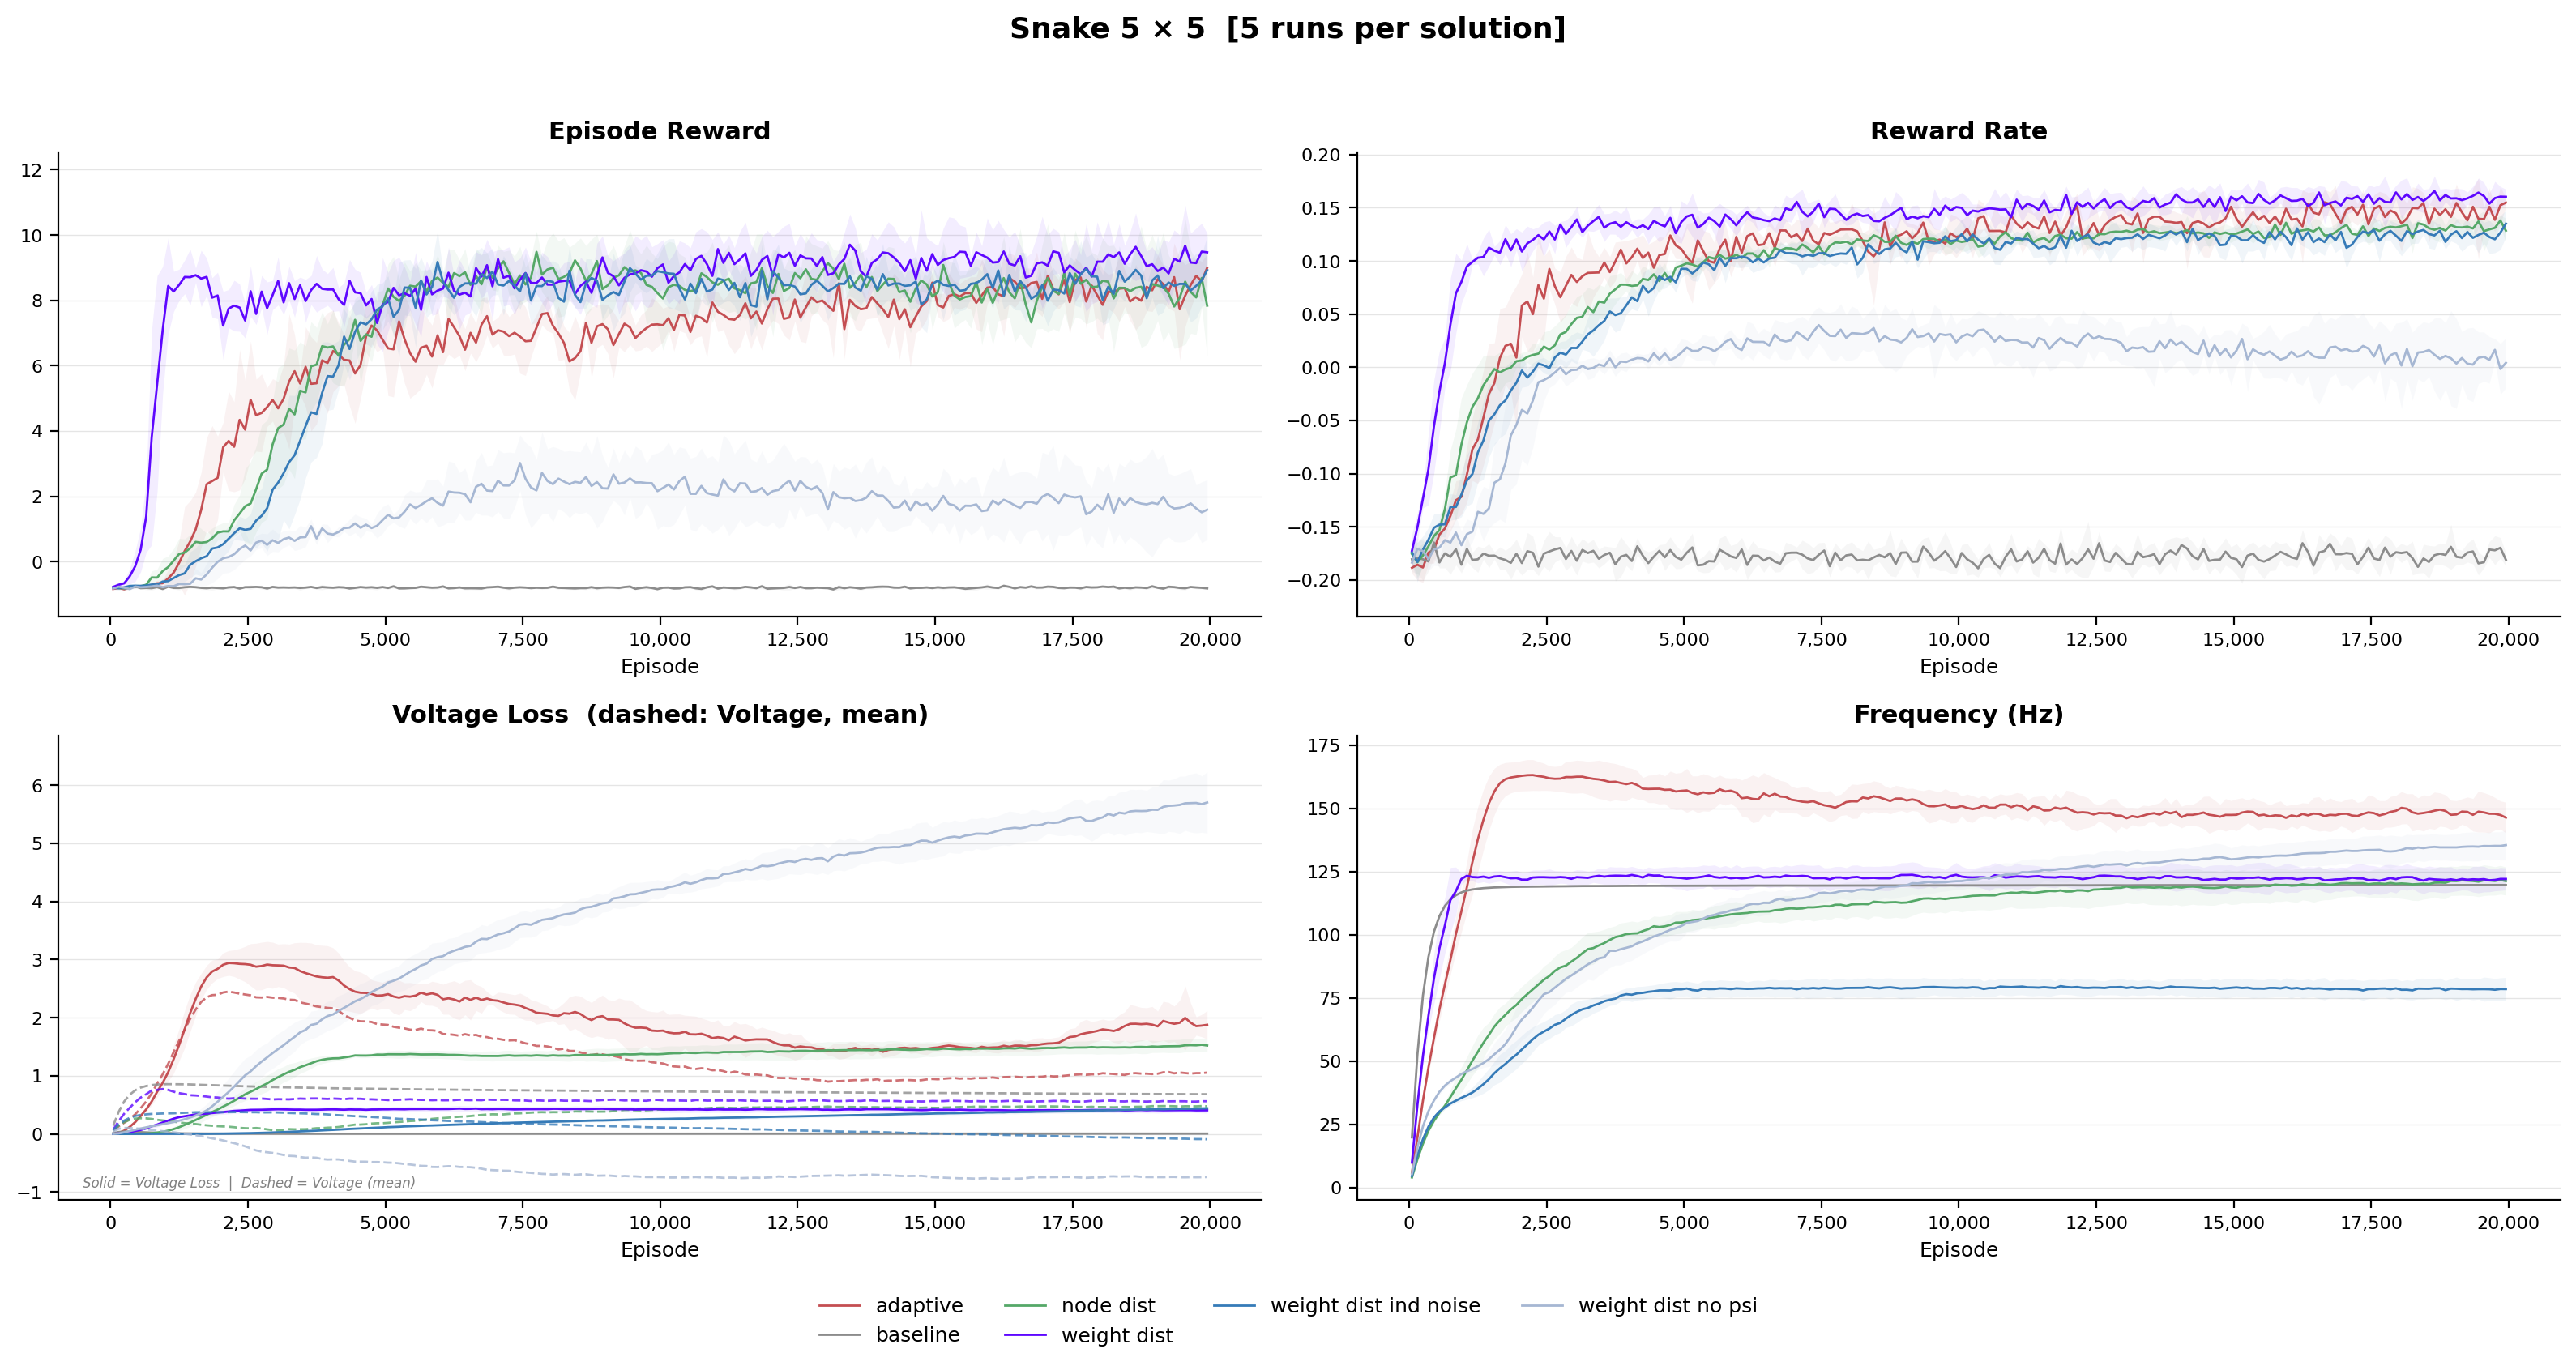
\includegraphics[width=0.98\textwidth]{images/comparison_misc_5_runs.png}
\caption{\textbf{\variant{weight dist} learns fastest and reaches the highest
reward rate on Snake.} Episode reward, reward rate, voltage-regularisation loss
(solid) with mean membrane voltage (dashed), and firing frequency over 20k
episodes; mean $\pm$ spread over five runs. The reservoir-inspired baseline is
activity-matched at $\approx 120$\,Hz.
\pending{: figure from pre-rerun pipeline, to be regenerated.}}
\label{fig:snake-comparison}
\end{figure*}

\begin{figure*}[t]
\centering
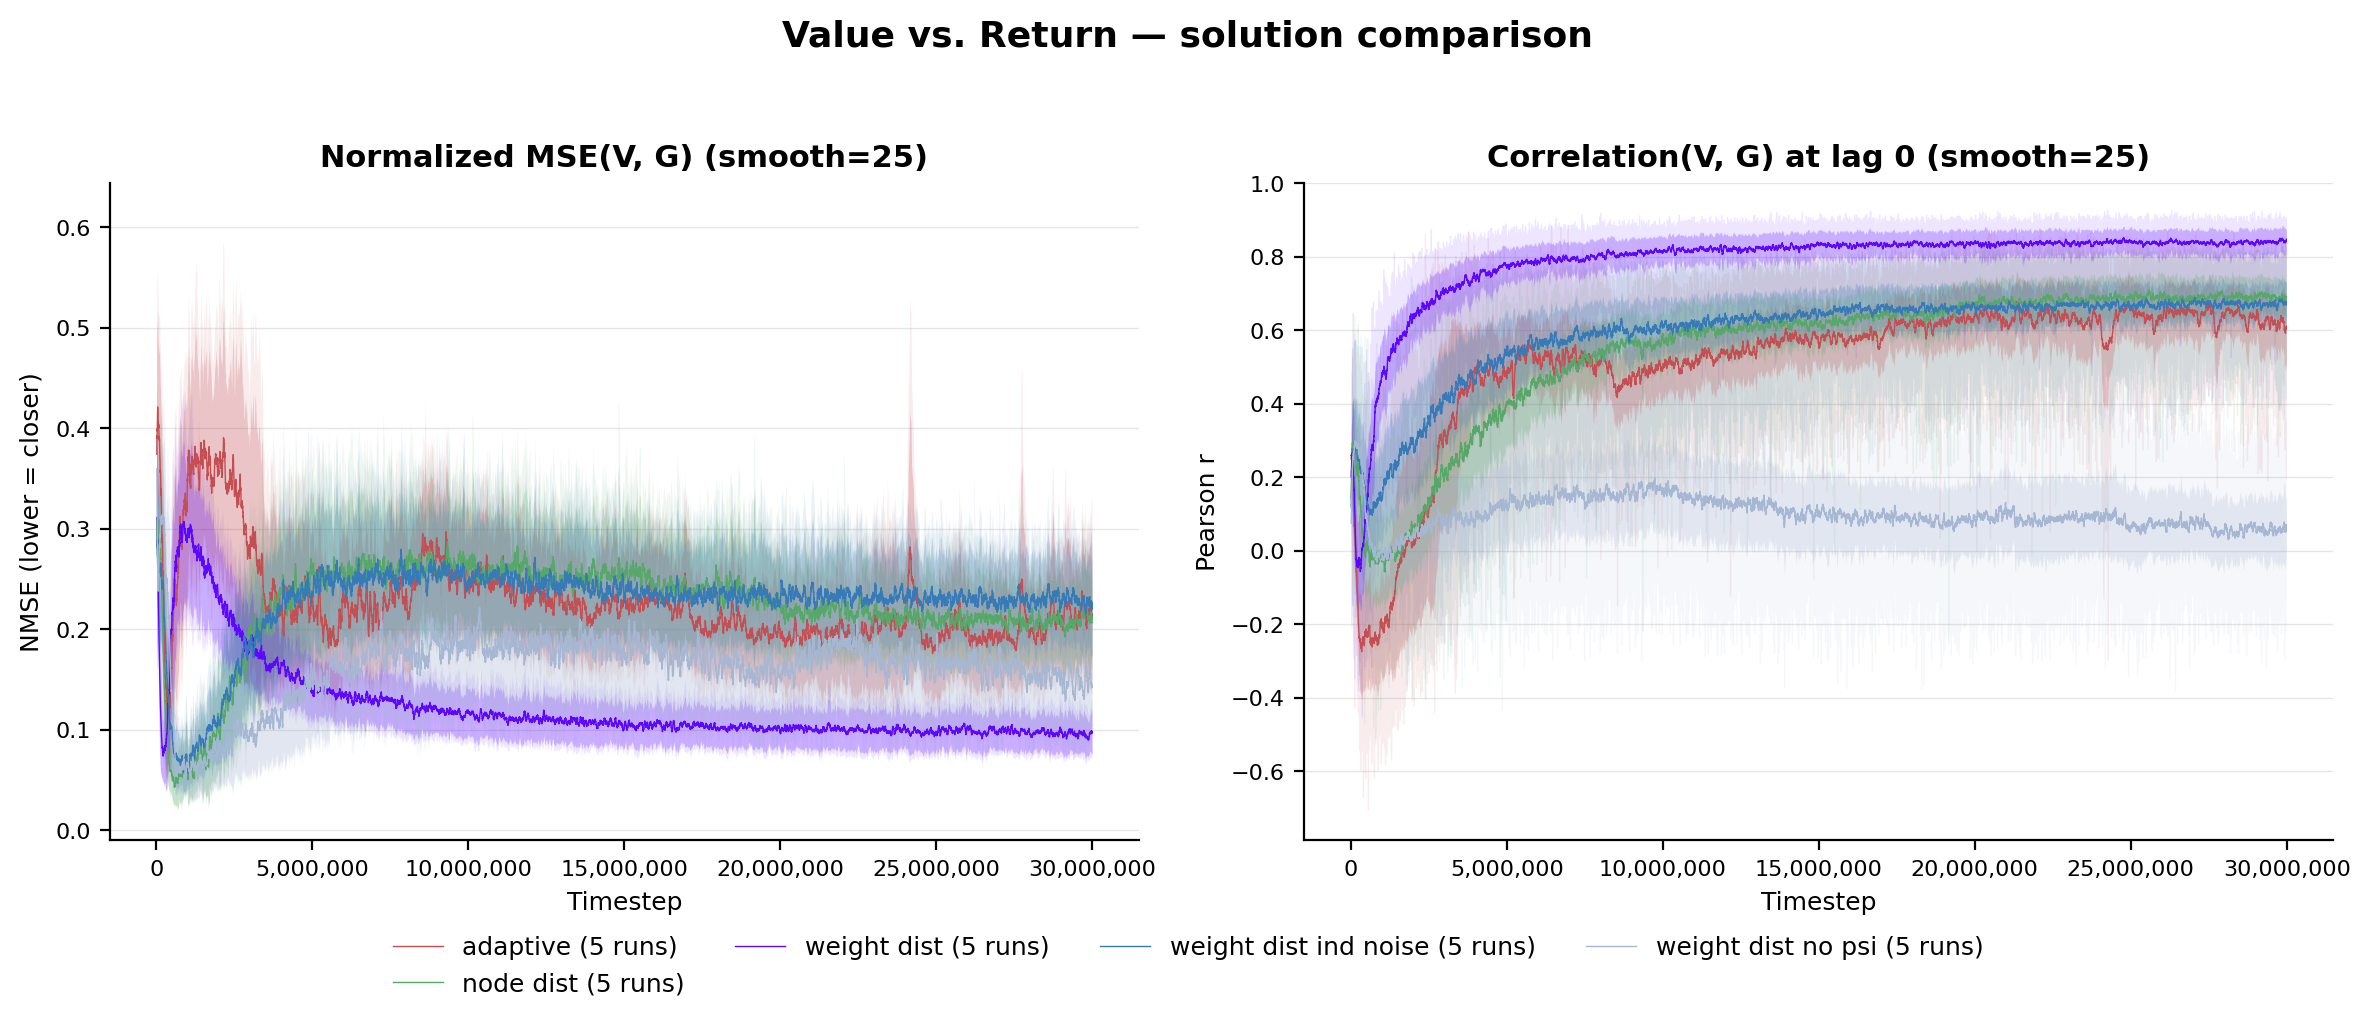
\includegraphics[width=0.9\textwidth]{images/snake_value_return_comparison.png}
\caption{\textbf{The \variant{weight dist} critic tracks the realised return
most closely.} Normalised squared error (left) and Pearson correlation (right)
between the critic's value $V_t$ and the realised return $G_t$ on Snake,
computed per window (Appendix~\ref{app:value-metrics}). Mean over five runs;
bands show $\pm 1$ s.d.\ and min--max; smoothed over 25 windows. 30M
simulation timesteps correspond to 1M environment steps.
\pending{: correspondence to the 20k-episode budget of
Fig.~\ref{fig:snake-comparison}.}}
\label{fig:snake-value-return}
\end{figure*}

\begin{figure*}[t]
\centering
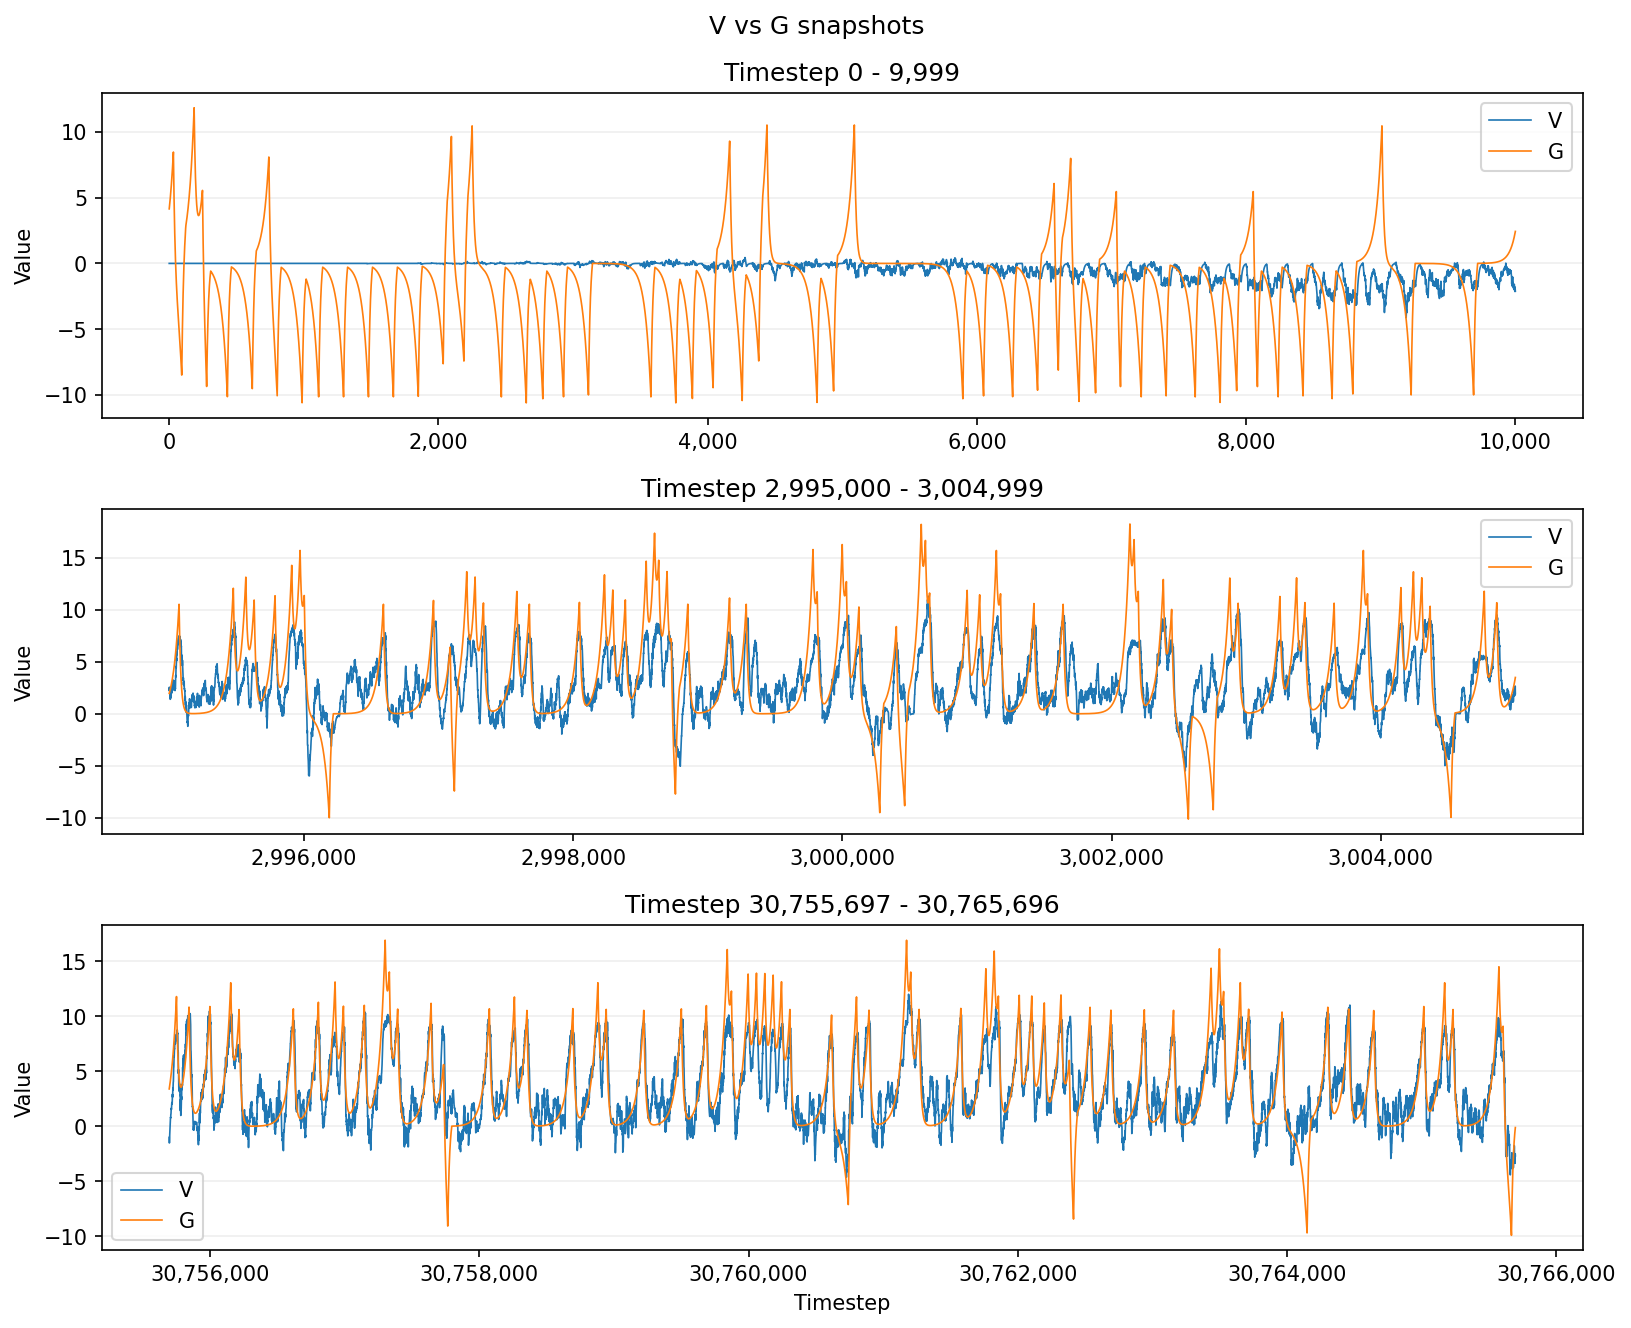
\includegraphics[width=0.49\textwidth]{images/snake_value_vs_g_weight_dist.png}\hfill
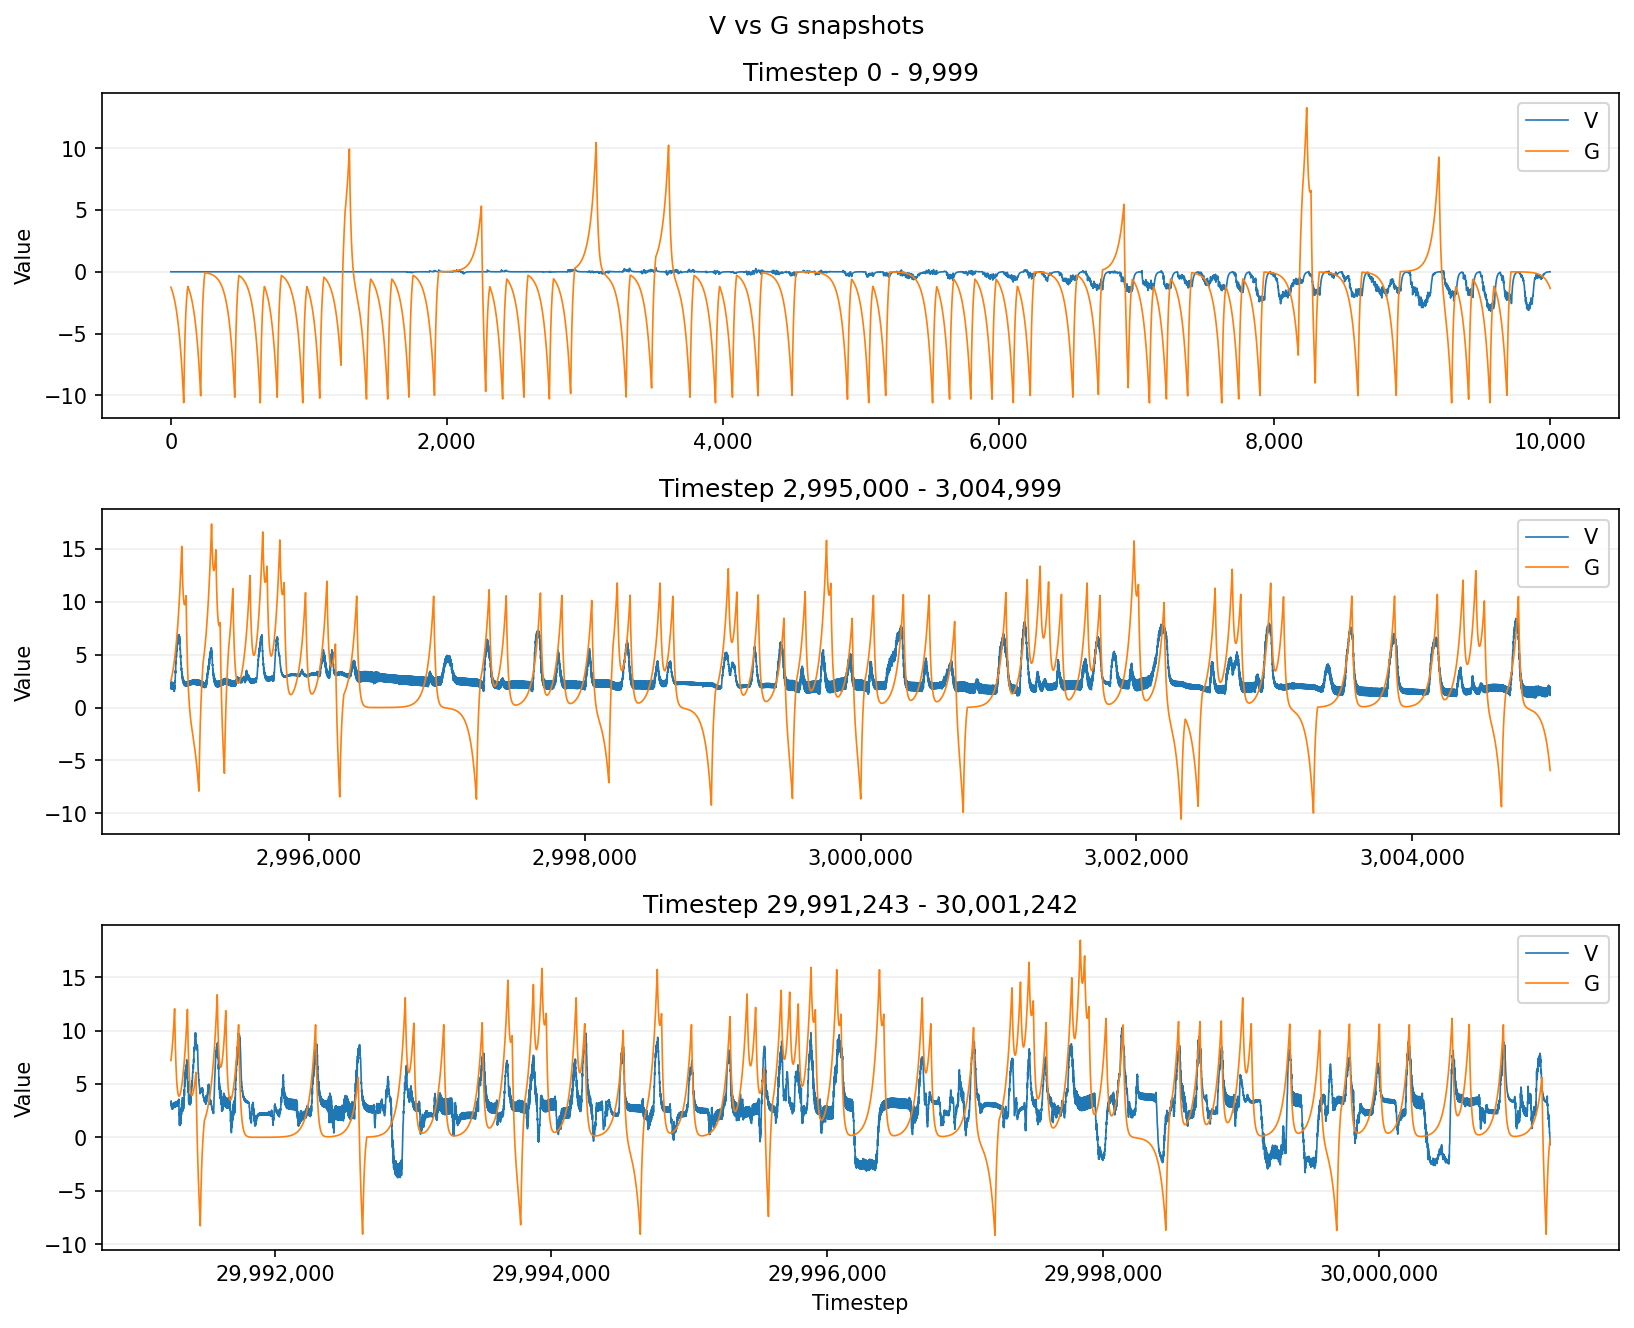
\includegraphics[width=0.49\textwidth]{images/snake_value_vs_g_adaptive.png}
\caption{\textbf{The \variant{weight dist} critic anticipates both food and
deaths; adaptive e-prop's misses most deaths.} Critic value $V_t$ (blue)
against the realised return $G_t$ (orange) in three 10k-timestep windows of one
run: start of training, around 3M timesteps, and end of training.
\emph{Left:} \variant{weight dist}; \emph{right:} adaptive e-prop.}
\label{fig:snake-vg-snapshots}
\end{figure*}

One calibration result frames the comparison. Symmetric e-prop is the
strongest configuration on Snake when the recurrent neurons connect directly
to the output heads, but it collapses to near-zero reward once per-head field
layers lengthen the causal path: its feedback weights are tied to the readout,
so neurons no longer directly connected to a head receive no feedback at all
(Appendix~\ref{sec:results-symmetric}).\pending{} This failure motivates the
two alternatives compared below, decoupling feedback from the forward weights
(adaptive e-prop) and removing structured feedback altogether (distributed
e-prop). All results that follow use the field layers.

\paragraph{Reading the two performance metrics.}
Episode reward and reward rate do not always rank the rules the same way.
Episode reward also credits simply surviving longer, whereas reward rate
measures how efficiently food is collected, which is the objective the
continuing task defines (Section~\ref{sec:results-ceiling}); we therefore rank
rules by reward rate. The distinction matters here: \variant{node dist} clearly
beats adaptive e-prop on episode reward, yet ends below it on reward rate
($\approx 0.13$ vs.\ $0.15$; Fig.~\ref{fig:snake-comparison}).

\paragraph{Overall comparison.}
Every learning rule except the ungated variant reaches episode reward
$\approx 8$--$9.5$, but the rules differ in speed and efficiency
(Fig.~\ref{fig:snake-comparison}). \variant{weight dist} is best throughout: it
reaches its plateau roughly five times sooner than any other rule and ends at
the highest reward rate ($\approx 0.16$). Adaptive e-prop rises more slowly but
ends second on reward rate, with the largest overshoot in voltage loss and
firing rate ($\approx 150$--$160$\,Hz). The reservoir-inspired baseline does not
learn at all. Its activity is matched to the learning rules and its recurrent
weights change only through the firing-rate regulariser, so its failure
indicates that task-driven learning in the recurrent weights is needed in these
experiments; a reservoir tuned for the task, as is usual in reservoir
computing, might fare better.

\paragraph{What makes distributed e-prop work.}
Comparing the distributed variants isolates two design choices. The first is
where the noise is injected. \variant{weight dist} and \variant{node dist} use
the same number of independent noise sources, yet \variant{weight dist}, whose
perturbation $\varepsilon^t_{ji}z^t_i$ is gated by presynaptic firing, learns
much faster and ends at a higher reward rate. \variant{weight dist ind noise}
keeps the per-synapse structure but multiplies the number of noise sources by
the fan-in, and learns about as slowly as \variant{node dist}. These results are
consistent with presynaptic gating making credit more specific and extra noise
sources adding variance, but because the perturbations depend on network
activity, the comparisons do not cleanly separate bias from variance, and we do
not attribute the gaps to either one. Structured routing adds nothing on top of
these variants (Appendix~\ref{app:routing}).

The second choice, the pseudo-derivative gate, matters most. Without it
(\variant{weight dist no $\psi$}) the rule barely learns, and its voltage
statistics show why the population mean alone can mislead: its voltage loss
climbs throughout training (to $\approx 5.7$) while its mean voltage settles
near $-0.75$, so individual membranes drift apart in both directions. Adaptive
e-prop's mean voltage, by contrast, tracks its voltage loss, a shift of the
whole population. The gate is therefore an essential part of the rule.

\paragraph{Critic quality.}
The critics differ as clearly as the policies. We compare each critic's value
$V_t$ with the discounted return $G_t$ realised along the continuing stream
(Appendix~\ref{app:value-metrics}), using the correlation to ask whether $V_t$
anticipates food and death events and a median-based NMSE for the prediction
error in a typical state. Both are relative to each rule's own policy, so they
mix critic quality with how hard that policy's return is to predict. The
\variant{weight dist} critic tracks the return most closely and earliest
($r\approx 0.84$, against $\approx 0.68$ for \variant{node dist} and
\variant{weight dist ind noise} and $\approx 0.62$ for adaptive e-prop;
Fig.~\ref{fig:snake-value-return}). The snapshots show the difference
(Fig.~\ref{fig:snake-vg-snapshots}): by about 3M timesteps \variant{weight dist}
follows $G_t$ through both food peaks and death dips, whereas adaptive e-prop's
value sits on a raised plateau and misses most death dips, which it only partly
captures by the end of training.

Every rule shows an early transient, a rise in error and a dip in correlation,
because the target is non-stationary: as the policy improves, the return shifts
from death-dominated to food-dominated, and the value must move from a
pessimistic to an optimistic estimate. The transient is shortest for
\variant{weight dist}, whose policy improves fastest, and longest and deepest
for adaptive e-prop. Without the gate, the value stays near zero and never
anticipates events; its moderate NMSE is nonetheless genuine, since its weak
policy produces a return that is mostly near zero and easy to predict. Finally,
critic accuracy does not settle the ranking on its own: adaptive e-prop has the
least accurate critic of the learning rules yet the second-best reward rate, so
a better critic accompanies, but does not guarantee, a better
policy.\pending{}


\subsection{Pac-Man}
\label{sec:results-pacman}

\pending{: new Pac-Man results to be added. Earlier Pac-Man results, under
the standard and the no-integration-during-refractory neuron models, are in
Appendix~\ref{sec:results-pacman-unmodified} and
Appendix~\ref{sec:results-pacman-nidrp}.}

% ===========================================================================
\section{Discussion}
\label{sec:discussion}
\pending{: interpretation below is based on the pre-rerun results and may
change once the AdaBelief/L2-Init runs land.}

\todo{Rewrite this section once the Pac-Man and Tic-Tac-Toe results are in.
It still carries thesis claims this paper does not show; every claim here
should point to a figure or table in this paper. (1) Remove claims with no
evidence here: ``worsening with causal path length'' and ``depth-robust''
(thesis depth experiments, not in the paper) and the ``self-limiting''
decoupled TD($\lambda$) sentence. Keep the voltage-shaping byproduct, but
rewrite it around the voltage-stability objective that is part of the method
(see the \todo in Section~\ref{sec:distributed}): the perturbation machinery
can optimise local, per-neuron objectives (voltage stability, voltage and
firing-rate regularisation), not only the broadcast TD error. Keep the claim safe:
local objectives are credited through the same perturbation correlation as the
TD error, and so in principle capture their dependence on the whole network.
Add, clearly marked as a \emph{hypothesis} and a main direction for future
work: reward-based (perturbation-credited) local objectives can relay richer
information than gradient-based ones. Gradient-based local objectives shape the
representation only with the context available along the local chain from
synapse to membrane (as in slowness and self-prediction learning, e.g.\ slow
feature analysis; neurons predicting their own future activity, Luczak et al.\
2022; Halvagal \& Zenke 2023 --- verify and add to the bibliography). Perturbation-credited
local objectives estimate, in expectation, the objective's total dependence on
each neuron's exploration, including effects mediated by the network, the
agent's actions and the environment, at the cost of extra variance; they could
therefore support local, action-dependent learning objectives, related in
spirit to active inference. Point to the voltage regulariser as a
\emph{possible} example: its gradient-based form made voltages diverge while
its perturbation-credited form did not, noting that $\psi$ is a confound. To
disentangle, run weight dist with the voltage regulariser (a) gradient-credited
without $\psi$ (thesis setup), (b) perturbation-credited with $\psi$ (current),
(c) gradient-credited gated by $\psi$: if (c) still diverges, the example
supports the hypothesis; if it is stable, $\psi$ explains it. Short runs
suffice. Optional experiment: adaptive e-prop with and without a gradient-based
voltage-stability term, to test whether it helps through the representation.
(2) Replace ``runaway voltage and firing'' for adaptive e-prop with what the
new data show (largest overshoot, which then settles). (3) Update the
Limitations: main results are now five seeds on three tasks; only the appendix
sweeps are single runs and use the earlier protocol; state that the
hyperparameter search was limited and shared by all rules. (4) Restructure:
main finding (broadcast scalar plus $\psi$ gate matches or beats adaptive
e-prop on all three tasks); what the analyses add (speed, reward rate, value
precision with its policy-dependence caveat, reservoir-inspired baseline);
bias--variance as one tentative reading, not the explanation; limitations,
including the action window. (5) Interpretation: present the perturbation trace $\xi$ and the $\psi$ gate as
the two essential components, with the $\psi$ and trace-vs-per-step ablations
as direct evidence. Treat the decoupled TD($\lambda$) separately, as shared
machinery that every rule in the paper depends on (not specific to the
$\xi$/$\psi$ argument); it is essential for anything here to work. Label the
remaining choices (AdaBelief, L2 Init, regularisers, shared-postsynaptic noise)
as supporting choices that improved stability in preliminary runs and were not
ablated. (6) End the
section with the spiking-synergy \emph{hypothesis}, clearly marked as such: the
spiking threshold makes the effect of exploration sparse and identifiable
(a perturbation matters only near threshold, which $\psi$ detects, and
perturbing the voltage itself lets $\xi$ measure how much of the current
deviation is exploration), so spiking may enable perturbation learning in the
strictly online setting rather than hinder it; a smooth, rate-based counterpart
(where the analogue of $\psi$ is never zero) is the direct test, left to
future work. Cite \citet{Lansdell2023}, who show that samples near the spiking
threshold give an unbiased estimate of a neuron's causal effect, as independent
support for the hypothesis. (7) Next to it, one or two sentences on the
estimator trade-off: the exact likelihood-ratio estimator is unbiased
precisely because it discards the known membrane propagation (conditioning on
the observed past leaves only the innovations $\varepsilon^t$ and the
instantaneous input), leaving that credit to be rediscovered through reward
correlations; the trace rule reintroduces this structure at the cost of bias.
An estimator that uses the known propagation and remains unbiased, e.g.\ via a
local control variate that removes the trace rule's bias, is an open problem
and a natural next step. (8) Summary of the variance-reduction interpretation, suggested wording:
``Taken together, the single-neuron analysis and the ablations suggest that
distributed e-prop trades a small bias for a substantial reduction in variance
relative to the exact perturbation estimator: its update stays within cosine
$0.97$--$0.99$ of the true gradient, while it is markedly less noisy whenever
neurons spend time silenced or saturated, and the exact estimator fails to
learn in the network. With a bias this small, we expect the rule's remaining
limitations to lie mainly on the side of noise, which for perturbation-based
credit is predicted to grow with the number of perturbed neurons; testing this
scaling directly is an important next step.'' (9) Outlook, clearly as
perspective: the noise term is driven by other neurons' perturbations reaching
the shared reward, so architecture could control it---sparse, modular
connectivity (cf.\ the sparsity of biological connectomes, e.g.\ the fruit-fly
connectome; verify and cite) and more local reward signals (per-module TD
errors, or the local rewards above) limit how much of that noise each neuron's
credit sees. Close with the broader view: distributed e-prop is not the whole
story, but it hints that perturbation learning---intrinsic noise, a broadcast
neuromodulator-like signal, and local eligibility---is a computationally
viable candidate for how brains could learn.}

The experiments show that, under strictly online, continuing constraints, a
rule with no structured feedback can match, and on Snake exceed, the strongest
e-prop variant, and that the two families differ in \emph{how} they learn. Adaptive e-prop is prone to pathological dynamics
(runaway voltage and firing, worsening with causal path length).
Distributed e-prop is well-regulated, learns better-structured value functions
(its value estimate correlates more strongly with the realised return,
Fig.~\ref{fig:snake-value-return}),
tolerates violations of the neuron model that break adaptive e-prop
(Appendix~\ref{sec:results-pacman-nidrp}), and looks
depth-robust at a fixed budget. Read together, these are two faces of one
bias--variance tradeoff: structured feedback pays a bias that accumulates with
path length but supplies a directed signal; perturbation-based credit trades
that directed signal for a noisy correlation, which the perturbation trace and
the $\psi$ gate make usable by exploiting known structure, at the cost of some
bias. Which is preferable is a genuine, task-dependent
question, not one with a fixed answer.

Two byproducts are worth highlighting. The perturbation trace lives in membrane
space and self-gates when the membrane is far from threshold, which makes local
\emph{voltage} reward shaping work in distributed e-prop where its standard
e-prop analogue diverges, suggesting a broader family of local objectives that
structured-feedback rules cannot easily support. The decoupled TD($\lambda$)
update likewise lets a short-horizon critic coexist with long-range credit,
though that reach is self-limiting once the critic is accurate.

\paragraph{Limitations.}
Several comparisons are single-seed and read as existence or relational
claims, not rankings; hyperparameters were not exhaustively tuned per rule.
All rules converge to firing rates of roughly $80$--$170$\,Hz, far above the
$10$\,Hz target and the biological range, plausibly because the reactive tasks
demand near-constant firing.\pending{: firing-rate range specific to
pre-rerun runs.} A systematic study
varying seeds, network size, task structure, and training length is needed to
turn these tendencies into settled claims.

The softmax policy head still
samples a discrete action at fixed action-window boundaries
(Appendix~\ref{app:impl}), requiring the network to consult an implicit
external clock, and the policy-gradient term of the learning signal is
delivered only at those sampling steps (in distributed e-prop, only to the
output weights). A genuinely clock-free agent would instead need a
continuously-defined action head, e.g.\ independent per-action Gaussian units
updated every timestep. We attempted many continuous action head
configurations, but found it substantially harder to stabilise than the
discrete softmax head. We suspect two properties of the softmax head, absent from independent
continuous units, may contribute to this gap. First, softmax's shared
normalisation couples the $A$ action logits' gradients into a single
mutually-exclusive distribution, so increasing one action's probability
mechanically decreases the others; independent action units carry no such
coupling and must learn any comparative structure among actions purely from
separate, per-unit signals. Second, the softmax head only requires a learning
signal at the specific timesteps an action is actually sampled, whereas a
continuously-defined head must be assigned credit at every timestep,
substantially increasing the surface over which credit must be correctly
apportioned. We leave a working continuous-action formulation to future work.
More broadly, the action window, and the per-action discount and trace decays
defined on it, are task-specific configuration that the learning rule could in
principle take over; moving as much of it as possible into the rule, towards a
fully task-agnostic agent, is the natural next step.
% ===========================================================================
\section{Conclusion}
\label{sec:conclusion}

\todo{Tighten to about four sentences after the Discussion rewrite: the
setting (few rules apply; e-prop as reference), the finding (distributed
e-prop matches or beats it on all three tasks, with the $\psi$ gate
essential), what it suggests (structured feedback may not be necessary in
this setting), and the next step (removing the action window and other
task-specific timing). Demote the decoupled TD($\lambda$) from headline to
supporting machinery, and mention the value-precision analysis and the
reservoir-inspired baseline. If the invariance of the update's magnitude to
path length and delay is mentioned (here or in the abstract), present it as a
property of e-prop-style local rules that distributed e-prop shares, not as
its distinguishing advantage over adaptive e-prop. Close with the spiking-synergy hypothesis from
the Discussion as an outlook, one sentence, marked as a hypothesis.}

Very few learning rules can train recurrent networks under strictly online,
continuing constraints, and e-prop is, we argue, the most promising of them.
We introduced distributed e-prop, a family of fully local, online learning
rules that trains recurrent spiking networks with reinforcement using only a
globally broadcast scalar and each neuron's own perturbation and eligibility
traces: no structured feedback weights of any kind. Paired with a decoupled
TD($\lambda$) rule for the non-episodic setting, its strongest variant matches
or exceeds adaptive-feedback e-prop, learning faster, reaching a higher reward
rate, and learning a more accurate critic,\pending{: summary claim pending
Pac-Man and Tic-Tac-Toe results.} while remaining expressible entirely as local
per-synapse updates suited to neuromorphic hardware. Its central lesson is that
a single global scalar \emph{can} drive effective learning in this setting when
paired with the right local gate, the e-prop pseudo-derivative. More broadly,
removing structured feedback altogether, rather than approximating it more
closely, turns out to be a competitive route to strictly online learning in
spiking networks. Understanding when and why, and removing the remaining
task-specific timing, above all the fixed action window, are the natural next
steps.

% ===========================================================================
\bibliographystyle{plainnat}
\bibliography{references}

\clearpage
% ===========================================================================
%  APPENDIX  (supplementary material; follows the references)
% ===========================================================================
\onecolumn
\appendix

\section{Network Architecture and Connectivity}
\label{app:arch}
The hidden core is a recurrent spiking network split into separate excitatory
(E) and inhibitory (I) populations respecting Dale's
principle~\citep{dale1935pharmacology,vanVreeswijk1996Chaos} at initialisation:
a $20\times20\times3$ E grid ($1200$ neurons) and a $15\times15\times3$ I grid
($675$ neurons), all adaptive leaky integrate-and-fire (ALIF) neurons.
Connections are sparse and spatially organised: each postsynaptic neuron samples
its afferents from a toroidal Gaussian profile over the normalised
sheet~\citep{Spreizer2019Toroidal}, with a wider reach for input projections
($\sigma_{\mathrm{in}}=0.1$) than for recurrent ones ($\sigma_{\mathrm{h}}=0.05$)
and a target fan-in of $K_{\mathrm{in}}\approx100$. Weights use a fan-in scaling
$1/\sqrt{K_{\mathrm{in}}}$;
excitatory connections take a small positive mean ($c_E=0.1$) and inhibitory a
larger magnitude ($c_I=3$) so that E and I drive are balanced despite the
smaller I population. The Dale sign is imposed only at initialisation and
released during training (a ``weakened'' Dale's law); enforcing it throughout,
or dropping the EI initialisation entirely, both impaired learning in our
experiments. The first is consistent with reports that naively enforcing
Dale's principle impairs learning~\citep{Cornford2021DaleANN}; see
\citet{Song2016DaleEI} for training recurrent networks with separate E and I
populations.

Each output head (policy and value) is optionally preceded by a dedicated,
non-recurrent \emph{field} population of the same shape as the I population,
which reads from the recurrent core and projects to a linear leaky-integrator
readout. By the \emph{causal path length} between a neuron and an output we mean
the shortest directed path in the connectivity graph; field layers increase it,
and we use them to test how gracefully each rule assigns credit as that path
grows.

\section{Implementation and Training}
\label{app:impl}
The network is implemented on the GPU-accelerated, event-driven, JIT-compiled
GeNN simulator~\citep{Yavuz2016GeNN} through its \texttt{ml\_genn} interface. All
per-synapse state (the filtered eligibility trace, the perturbation trace, and,
in the distributed variants, the per-synapse $\log\sigma_{ji}$) is stored on
device and updated in a single fused kernel, so each update is a local
read--modify--write with no backward sweep; this scales to $\sim$1{,}900 neurons
and millions of synapses. Training is \emph{strictly online} and
\emph{continuing} (Section~\ref{sec:intro}): the environment's ending signal
resets the environment but never the network, so membrane potentials,
adaptation, and all traces persist across game boundaries. Each environment step
spans $K=30$ integration steps ($\Delta t = 1$\,ms); observations are converted
to spikes by independent Bernoulli sampling with per-pixel probability
proportional to intensity up to $p_{\max}$. Weights are updated with batch size
$1$ every simulation timestep, throughout, for every rule and on every task.
Section~\ref{sec:intro} explains why: choosing a coarser schedule means
deciding in advance, per task, where enough evidence has accumulated to
justify an update, and we have no general, task-agnostic rule for making that
choice. Updating every timestep sidesteps that decision
entirely.\pending{: the results in Appendix~\ref{app:extra-results} predate
the current configuration: they used plain Adam, no L2 Init, and, on Pac-Man,
per-episode updates.}

\paragraph{Value-precision metrics.}
\label{app:value-metrics}
To measure how well a critic predicts what actually happens, we log its value
$V_t$ and the reward signal $r_t$ at every simulation timestep and compute the
realised discounted return with a single backward pass over the whole
uninterrupted run,
\begin{equation}
G_t = r_t + \gamma_{\mathrm{step}}\, G_{t+1},
\qquad \gamma_{\mathrm{step}} = \gamma^{1/K},
\label{eq:realised-return}
\end{equation}
so that $\gamma=0.5$ per environment step is spread over its $K=30$
integration steps. As in training, game boundaries do not reset the return,
which matches the continuing objective. Each run, truncated to 30M timesteps,
is split into non-overlapping windows $w$ of
$W$\pending{: window size $W$ to be confirmed} timesteps, and in each window we compute
\begin{equation}
\mathrm{NMSE}_w = \operatorname*{median}_{t\in w}
\frac{(V_t - G_t)^2}{\operatorname{Var}_{w}(G)},
\qquad
r_w = \operatorname{corr}_{t\in w}(V_t, G_t),
\label{eq:value-metrics}
\end{equation}
the latter being the Pearson correlation at lag zero. Across the five runs of
each variant we report, per window, the mean, a $\pm1$ s.d.\ band, and the
min--max band; for plotting only, the series are smoothed with a centred moving
average over 25 windows (rolling extrema for the correlation's min--max band).
The median makes $\mathrm{NMSE}_w$ a robust summary of the prediction error in
a typical state, whereas $r_w$ is driven by whether $V_t$ anticipates the food
and death events. Both are computed against the return generated by each rule's
own policy, so they are not independent of policy quality: a stable, weak
policy can produce a return that is easier to predict than that of a policy
still improving, whose return is a moving target for the critic. The snapshots of
Fig.~\ref{fig:snake-vg-snapshots} show raw $V_t$ and $G_t$ over 10k-timestep
windows of a single run, the first and last anchored to the start and end of
that run and the middle one placed at 3M timesteps.

\section{Single-Neuron Analysis of the Perturbation Estimators}
\label{app:trace}

This appendix characterises the bias and noise of the perturbation-based
updates of Section~\ref{sec:distributed} in a setting where the true gradient
can be computed. All scripts are available in the repository
(\texttt{derivations/estimator\_toy}).\todo{Replace the repository path by the
public code link before submission.}

\subsection{Setup}
\label{app:trace-setup}

We simulate a single ALIF neuron with the dynamics and parameters of
Appendices~\ref{app:arch} and~\ref{app:hyper} ($\alpha=e^{-1/10}$, relative
reset, a refractory period of three steps, threshold adaptation, and e-prop's
pseudo-derivative $\psi$). Ten presynaptic inputs fire with probability $0.7$
per step during active periods separated by silent gaps. Perturbations use the
magnitudes of the experiments: $\sigma_j=e^{-4.61}$ for membrane (node) noise
and $\sigma_{ji}=e^{-5}$ for synaptic noise. The reward mimics the tasks: every
$K=30$ steps is an action window, and at a sparse random subset of windows a
reward event $R=\pm\tanh((y-\theta)/0.5)$ occurs, where $y$ is a leaky readout of
the neuron's spikes and the threshold $\theta$ and sign vary per event; the
reward is delivered as a decaying trace $r_t$. Every estimator uses causal
credit through the actor's trace, $p^t=\lambda\,p^{t-1}+c^t$ with
$\lambda=0.8^{1/K}$, and is read out as $\sum_t (r_t-b_t)\,p^t$ with a baseline
$b_t$. The truth is the exact estimator below with cumulative causal credit,
which is unbiased; we cross-checked it against central finite differences with
common random numbers (agreement to cosine $\ge 0.999$ whenever the difference
step is small compared with the noise's effect on the membrane). We report the
cosine between each estimator's mean and the truth, and its relative noise
$\sqrt{\mathrm{tr}\,\mathrm{Cov}}/\lVert\text{mean}\rVert$ per sample, which is
independent of the learning rate; the number of samples needed for a given
precision scales with its square.

For the weight-dist placement used by the main rule, the per-step contribution
$c^t_{ji}$ of each estimator is

\begin{center}
\footnotesize
\begin{tabular}{@{}ll@{}}
\toprule
estimator & $c^t_{ji}$ \\
\midrule
distributed e-prop & $(1-\alpha^2)\,\xi^t_{ji}/\sigma_{ji}^2\cdot e^t_{ji}$ \\
trace, no $\psi$ & $(1-\alpha^2)\,\xi^t_{ji}/\sigma_{ji}^2\cdot \bar z^t_i$ \\
per-step, with $\psi$ & $\eta^t_{ji}/\sigma_{ji}^2\cdot e^t_{ji}$ \\
per-step, presynaptic trace & $\eta^t_{ji}/\sigma_{ji}^2\cdot \bar z^t_i$ \\
exact & $\varepsilon^t_j\, z^{t-1}_i \big/ \textstyle\sum_k \sigma_{jk} z^{t-1}_k$ \\
\bottomrule
\end{tabular}
\end{center}

\noindent where $\eta^t_{ji}=\sigma_{ji}\varepsilon^t_j z^{t-1}_i$ is the
perturbation synapse $ji$ applies (only on a presynaptic spike, with one
$\varepsilon^t_j\sim\mathcal N(0,1)$ shared by the neuron's synapses),
$\xi^t_{ji}=\alpha\,\xi^{t-1}_{ji}+\eta^t_{ji}$ is its per-synapse trace, and
$e^t_{ji}$ is e-prop's eligibility trace, as in the implementation.

\subsection{The exact estimator}
\label{app:trace-exact}

For membrane noise, $v^t=\alpha v^{t-1}+\sum_i W_{ji}z^{t-1}_i-v_{\mathrm{th}}z^{t-1}+\varepsilon^t$,
the probability of the sampled trajectory factorises into one-step Gaussians
around $\mu^t=\alpha v^{t-1}+\sum_iW_{ji}z^{t-1}_i-v_{\mathrm{th}}z^{t-1}$, in
which the previous, sampled membrane is fixed. The score is therefore
$\sum_t\varepsilon^t z^{t-1}_i/\sigma^2$: each perturbation is scored once,
at the step it was injected, and its lasting effect on the membrane, spikes,
and rewards is credited through the return. Because each neuron's noise is
independent and spikes are deterministic given the membranes, summing these
scores gives the exact likelihood-ratio gradient of the whole recurrent
network.

The same estimator can be written around the noise-free trajectory,
$v=\bar v(W)+\xi$. The perturbations then form a first-order autoregressive
process with covariance $\Sigma$, and the score is
$(\partial\bar v/\partial W_{ji})^{\!\top}\Sigma^{-1}\xi=\bar z_i^{\top}\Sigma^{-1}\xi$.
The synaptic drive and the perturbations pass through the \emph{same} membrane
filter, so the transform $L$ that decorrelates the perturbations
($L\xi=\varepsilon$, with $\Sigma^{-1}=L^{\top}L/\sigma^2$) is the inverse of
that filter. Splitting it between the two factors,
$\bar z_i^{\top}\Sigma^{-1}\xi=(L\bar z_i)^{\top}(L\xi)/\sigma^2$, also
un-integrates the eligibility ($L\bar z_i=z_i$) and recovers the step-wise form.
The trace rule instead pairs $\xi$ with $\bar z$ directly, i.e.\ it replaces
$\Sigma^{-1}$ by its diagonal, treating successive values of $\xi$ as
independent.

For the noise placements of Section~\ref{sec:distributed} the exact score is,
analogously, the perturbation that reaches the membrane divided by its
variance at that step, times the presynaptic spike. For shared synaptic noise
(weight dist) the membrane perturbation is
$\varepsilon^t_j\sum_i\sigma_{ji}z^{t-1}_i$, whose variance changes with which
inputs fired, which gives the entry in the table above; for independent
synaptic noise it is the classical weight-perturbation score
$\eta^t_{ji}/\sigma_{ji}^2$.

\subsection{Bias of the trace rule}
\label{app:trace-bias}

Write $g_s=\mathbb E[\partial F/\partial v^s]$ for the sensitivity of the
reward to the membrane at step $s$; the true gradient is
$\sum_s g_s\bar z^s_i$. For Gaussian perturbations, Stein's lemma,
$\mathbb E[F\xi]=\Sigma\,\mathbb E[\nabla_vF]$, gives the expectation of the
(ungated) trace rule as
\begin{equation}
\mathbb E\Big[F\sum_t\tfrac{(1-\alpha^2)}{\sigma^2}\,\xi^t\bar z^t_i\Big]
=\sum_s g_s\,\tilde z^s_i,\qquad
\tilde z^s_i=\sum_t\alpha^{|t-s|}\,\bar z^t_i ,
\label{eq:trace-bias}
\end{equation}
in the stationary regime. The trace rule is thus the exact gradient with the
presynaptic trace blurred by the correlation kernel of the perturbations,
whose width is the membrane time constant. For a reward at a single final step
this reduces to weighting input $x^{r-1}$ by an extra factor $T-r+1$: a
perturbation is credited through its correlation with the return and again
through its lingering contribution to every later $\xi^t$. For a constant input
the two expectations differ only by a factor $1/(1-\alpha)$, absorbed by the
learning rate. In general the blur costs little when the reward's sensitivity
to the membrane varies slowly compared with $\tau_{\mathrm{mem}}$ and more when
it varies faster: in a leaky neuron with random input spikes, the cosine between
Eq.~\eqref{eq:trace-bias} and the true gradient averaged $0.999$, $0.98$,
$0.94$, and $0.89$ for sensitivities that vary on scales of $100$, $30$, $10$,
and $1$ steps. We verified Eq.~\eqref{eq:trace-bias} by Monte Carlo, both in a
leaky neuron and with the full ALIF dynamics.

\subsection{Noise}
\label{app:trace-noise}

Each estimator's score is linear in the innovations,
$S_i=a_i^{\top}\varepsilon$, with a \emph{score profile} $a_i$ fixed by the
rule. For small noise the reward fluctuation is approximately linear too,
$F-\mathbb E[F]\approx g_\varepsilon^{\top}\varepsilon$, where
$g_{\varepsilon,s}=\sum_{t\ge s}\alpha^{t-s}g_t$ is the reward's sensitivity to
the perturbation injected at step $s$. Gaussian moments (Isserlis' theorem)
then give the mean $\sigma^2 g_\varepsilon^{\top}a_i$ and the relative noise
\begin{equation}
\text{relative noise}^2
=1+\frac{\lVert g_\varepsilon\rVert^2\sum_i\lVert a_i\rVert^2}{\sum_i\big(g_\varepsilon^{\top}a_i\big)^2}.
\label{eq:noise-formula}
\end{equation}
The relative noise depends neither on $\sigma$ nor on the reward's scale, only
on how well each synapse's score profile aligns with the reward's sensitivity
to the noise. Both are forward-filtered by the membrane: the trace $\xi$ gives
the score profile the same filter, $a_s\propto\sum_{t\ge s}\alpha^{t-s}\bar z^t$,
whereas the exact estimator's profile is the raw input. The gate $\psi$,
evaluated on the noise-free trajectory, enters as a deterministic reweighting
of the profile; this is accurate because its width ($v_{\mathrm{th}}$) is about
forty times the perturbations' effect on the membrane. With the full ALIF
dynamics and a per-step reward, Eq.~\eqref{eq:noise-formula} predicted every
estimator's direction to within $0.001$ in cosine, and bracketed its measured
relative noise between the value computed from the reward's linear part
(below) and the value obtained by replacing $\sigma^2\lVert g_\varepsilon\rVert^2$
by the total reward variance (above, within $7\%$); only $57\%$ of the reward's
variance was linear in the noise, the rest coming from discrete spike flips.

\subsection{Results}
\label{app:trace-results}

Table~\ref{tab:toy-regimes} reports the five estimators for the weight-dist
placement across operating regimes, set by the input weights: near threshold
(the baseline), silenced by inhibitory inputs, and saturated. We omit a
strongly saturated regime, in which the reward barely depends on the neuron
and the truth itself could not be estimated reliably.

\begin{table}[h]
\centering\footnotesize
\begin{tabular}{@{}lccccccc@{}}
\toprule
regime & firing & $\psi$ open & dist.\ e-prop & trace, no $\psi$ & per-step, $\psi$ & per-step, pre.\ trace & exact \\
\midrule
near threshold          & 15.5\% & 68\% & 0.993\,/\,8.2 & 0.990\,/\,6.8 & 0.991\,/\,7.2 & 0.989\,/\,5.7 & 0.999\,/\,6.9 \\
inhibited (34\% far below) & 4.0\% & 60\% & 0.980\,/\,2.7 & 0.992\,/\,3.7 & 0.972\,/\,2.6 & 0.991\,/\,3.1 & 1.000\,/\,3.9 \\
inhibited (64\% far below) & 3.4\% & 31\% & 0.977\,/\,2.7 & 0.986\,/\,5.7 & 0.986\,/\,2.8 & 0.980\,/\,4.6 & 1.000\,/\,5.7 \\
saturated (39\% far above) & 27.6\% & 29\% & 0.974\,/\,3.1 & 0.986\,/\,4.9 & 0.945\,/\,3.0 & 0.975\,/\,4.3 & 0.999\,/\,4.1 \\
\bottomrule
\end{tabular}
\caption{Single-neuron estimators, weight-dist placement (shared synaptic noise,
per-synapse traces), sparse decaying reward, $\lambda$ credit, $400$k samples
per regime. Each cell gives the cosine to the true gradient and the relative
noise per sample. ``Far below/above'' means more than $v_{\mathrm{th}}$ from the
adaptive threshold. The uncertainty of the truth is at most $1.7\%$.}
\label{tab:toy-regimes}
\end{table}

Three observations follow. First, every update is only slightly biased:
all point within cosine $0.97$--$0.99$ of the true gradient in every regime.
Second, $\psi$ reduces the noise when the neuron spends time where its
perturbations cannot change a spike, by a factor $1.4$--$2.1$ when silenced or
saturated, and there the gated rules are less noisy than the exact estimator;
near threshold, where $\psi$ is open most of the time, it slightly increases the
noise, and it does not improve the direction in this setting. Third, with
per-synapse traces the trace does \emph{not} reduce the noise relative to
per-step perturbations (compare distributed e-prop with ``per-step, $\psi$''),
although in the network the per-step variant learns more slowly
(Section~\ref{sec:results-snake}).\pending{: Snake ablation.} The advantages
of the trace and the gate observed in networks therefore go beyond what a
single neuron shows. With neuron-level (membrane) noise, in contrast, the trace
rule was less noisy than the exact estimator and far more robust than the
per-step rule to a narrower gate.

Table~\ref{tab:toy-placement} compares the noise placements, each with its own
trace rule and exact estimator. Which placement is less noisy depends on the
regime. Near threshold with dense input, membrane noise is about three times
less noisy than shared synaptic noise; when the neuron is often silenced, the
order reverses and shared synaptic noise is about seven times less noisy.
Membrane noise is injected at every step, including the many steps at which a
silenced neuron's perturbation cannot matter, and so adds reward variance that
no synapse's score can account for; synaptic noise enters only through
synapses that just carried a spike.

\begin{table}[h]
\centering\footnotesize
\begin{tabular}{@{}lcccc@{}}
\toprule
& \multicolumn{2}{c}{near threshold} & \multicolumn{2}{c}{inhibited (64\% far below)} \\
placement & trace rule & exact & trace rule & exact \\
\midrule
node (membrane noise)      & 0.993\,/\,2.8 & 0.999\,/\,3.8 & 0.855\,/\,19.6 & 0.958\,/\,25.7 \\
weight dist (shared)       & 0.993\,/\,8.2 & 0.999\,/\,6.9 & 0.977\,/\,2.7 & 1.000\,/\,5.7 \\
ind.\ noise (independent)  & 0.948\,/\,8.8 & 0.998\,/\,8.2 & 0.970\,/\,9.7 & 0.999\,/\,17.2 \\
\bottomrule
\end{tabular}
\caption{Noise placement, same setting as Table~\ref{tab:toy-regimes}; cells
give cosine to the true gradient and relative noise. The truth's uncertainty is
at most $1.7\%$, except for the inhibited node row ($5.5\%$, cosine about
$\pm0.05$).}
\label{tab:toy-placement}
\end{table}

\subsection{Limitations}
\label{app:trace-limits}

The analysis concerns a single neuron with a synthetic reward and no critic;
the reward is credited through the actor's trace but not through a learned TD
error. It measures how well each update estimates the gradient, not how well a
network learns with it, and it does not reproduce the network-level effects of
Section~\ref{sec:results-snake}, where removing $\psi$ breaks learning.


\section{Additional Results: Objective Horizon and Symmetric Feedback}
\label{app:extra-results}

\subsection{The Objective Horizon is Set by \texorpdfstring{$\gamma$}{gamma}, not \texorpdfstring{$\lambda$}{lambda}}
\label{sec:results-ceiling}

On Snake $5\times5$, the PPO reference makes the two performance metrics
concrete. With a long horizon ($\gamma=0.99$) the episodic and continuing
objectives diverge sharply (episode reward $\approx 22$ vs.\ reward rate
$\approx 0.24$, each poor on the other's metric), confirming that reward rate
and episodic return are genuinely different targets. At the short horizon the
spiking rules require ($\gamma=0.5$), both objectives collapse onto the same
compromise (episode reward $\approx 13$, reward rate $\approx 0.2$;
Fig.~\ref{fig:ppo}), because the
$\approx$2-step value horizon cannot represent either extreme. Crucially, the
continuing PPO run lands essentially where symmetric e-prop
does\pending{: symmetric e-prop number pre-rerun; PPO itself unaffected}: a
strong gradient optimiser given the identical short-horizon objective reaches
the same operating point as the local spiking rule. The spiking results are
therefore limited by the objective horizon, not by their credit-assignment
machinery, and decoupling $\lambda$ (Section~\ref{sec:tdlambda}) can extend the
effective policy horizon only where the critic cannot already predict the
relevant rewards.

\begin{figure}[H]
\centering
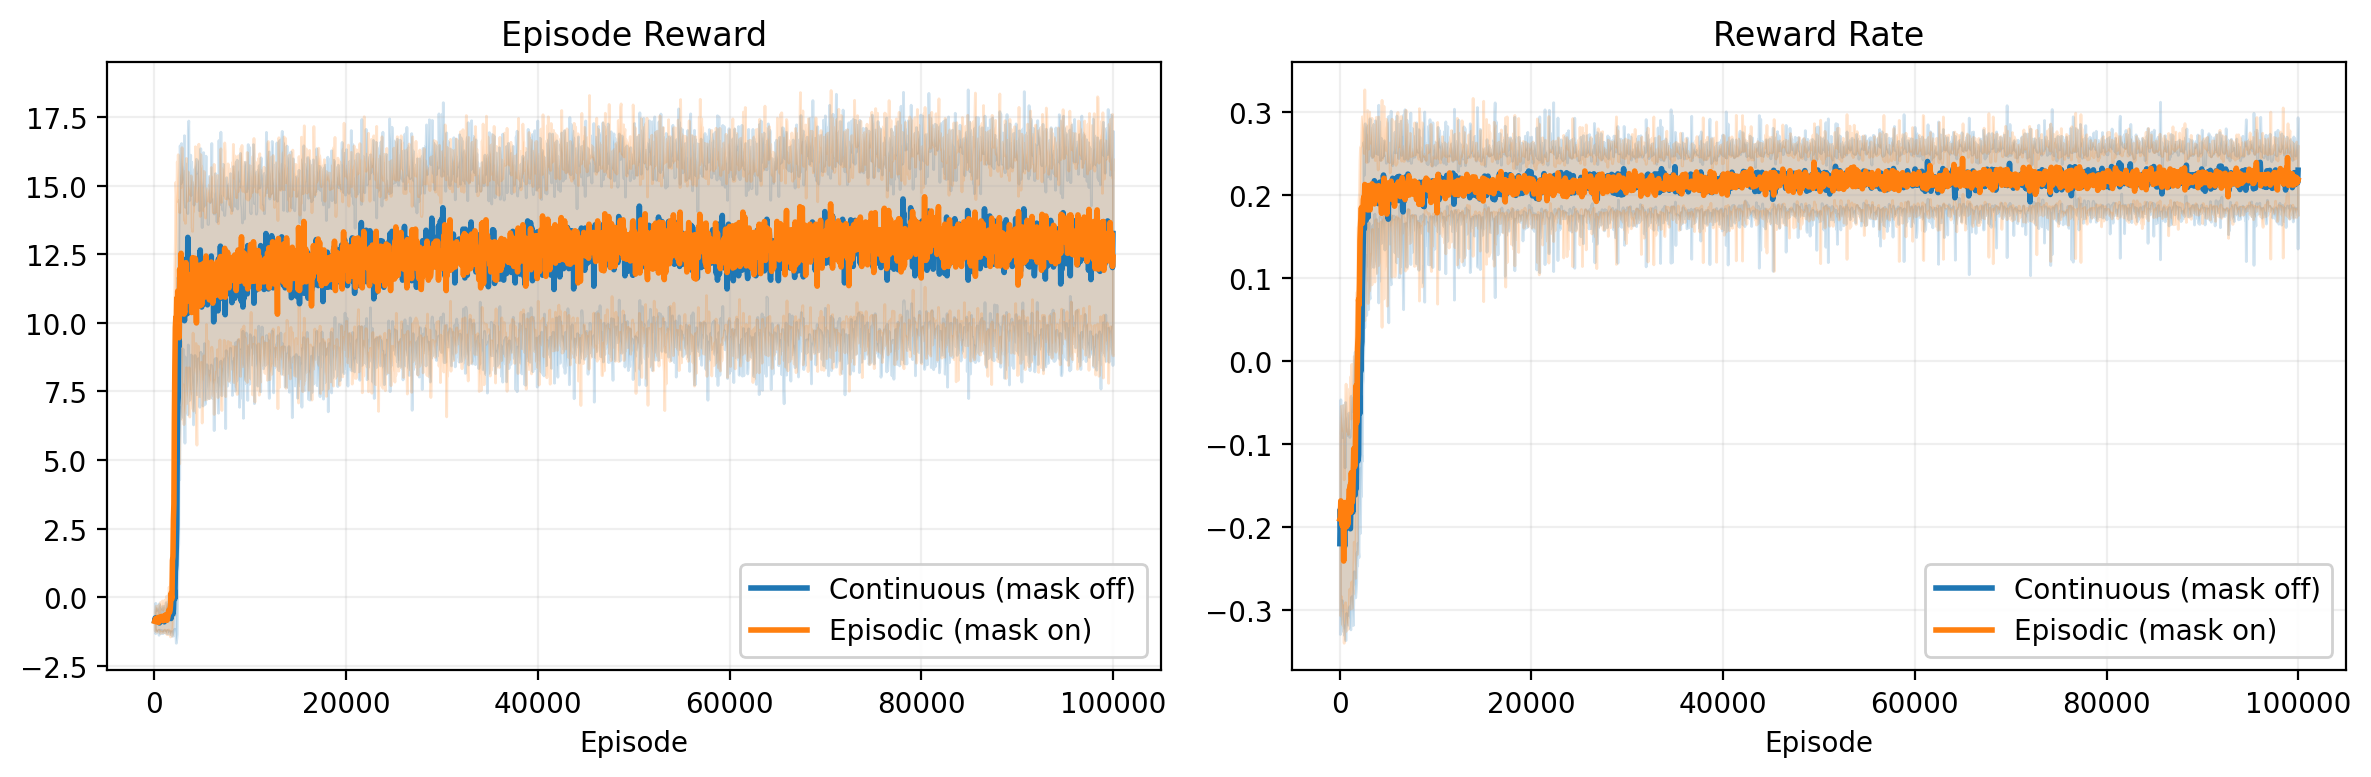
\includegraphics[width=0.95\linewidth]{images/PPOComparison.png}
\caption{PPO on Snake $5\times5$ under the episodic (terminal mask on) and
continuing (terminal mask off) objectives, both at the decoupled setting
$\gamma=0.5$, $\lambda=0.8$ used by the spiking rules. \emph{Left:} episode
reward; \emph{right:} reward rate. At this short value horizon the two
objectives nearly coincide on both metrics, and the continuing run lands where
symmetric e-prop does. (At $\gamma=0.99$, not shown, the two objectives instead
diverge to $\approx 22$ vs.\ $\approx 0.24$ on their respective metrics.)}
\label{fig:ppo}
\end{figure}

\subsection{Symmetric E-prop Excels but Fails as the Causal Path Grows}
\label{sec:results-symmetric}

Symmetric e-prop is the single strongest configuration on Snake, reaching the
highest reward and reward rate with the healthiest voltage and frequency
statistics (Fig.~\ref{fig:symmetric}). But introducing the per-head field layers collapses it to near-zero
reward: because its feedback weights are tied to the forward readout, neurons
that are no longer directly connected to a head receive \emph{no} feedback once
the causal path length exceeds one. Qualitatively, both the value trace and the
policy lose all structure. This is not a gradual degradation but an outright
failure mode, and it is precisely what motivates the two escape routes we
study: decoupling feedback from the forward weights (adaptive e-prop) and
removing structured feedback altogether (distributed e-prop).\pending{}

\begin{figure}[H]
\centering
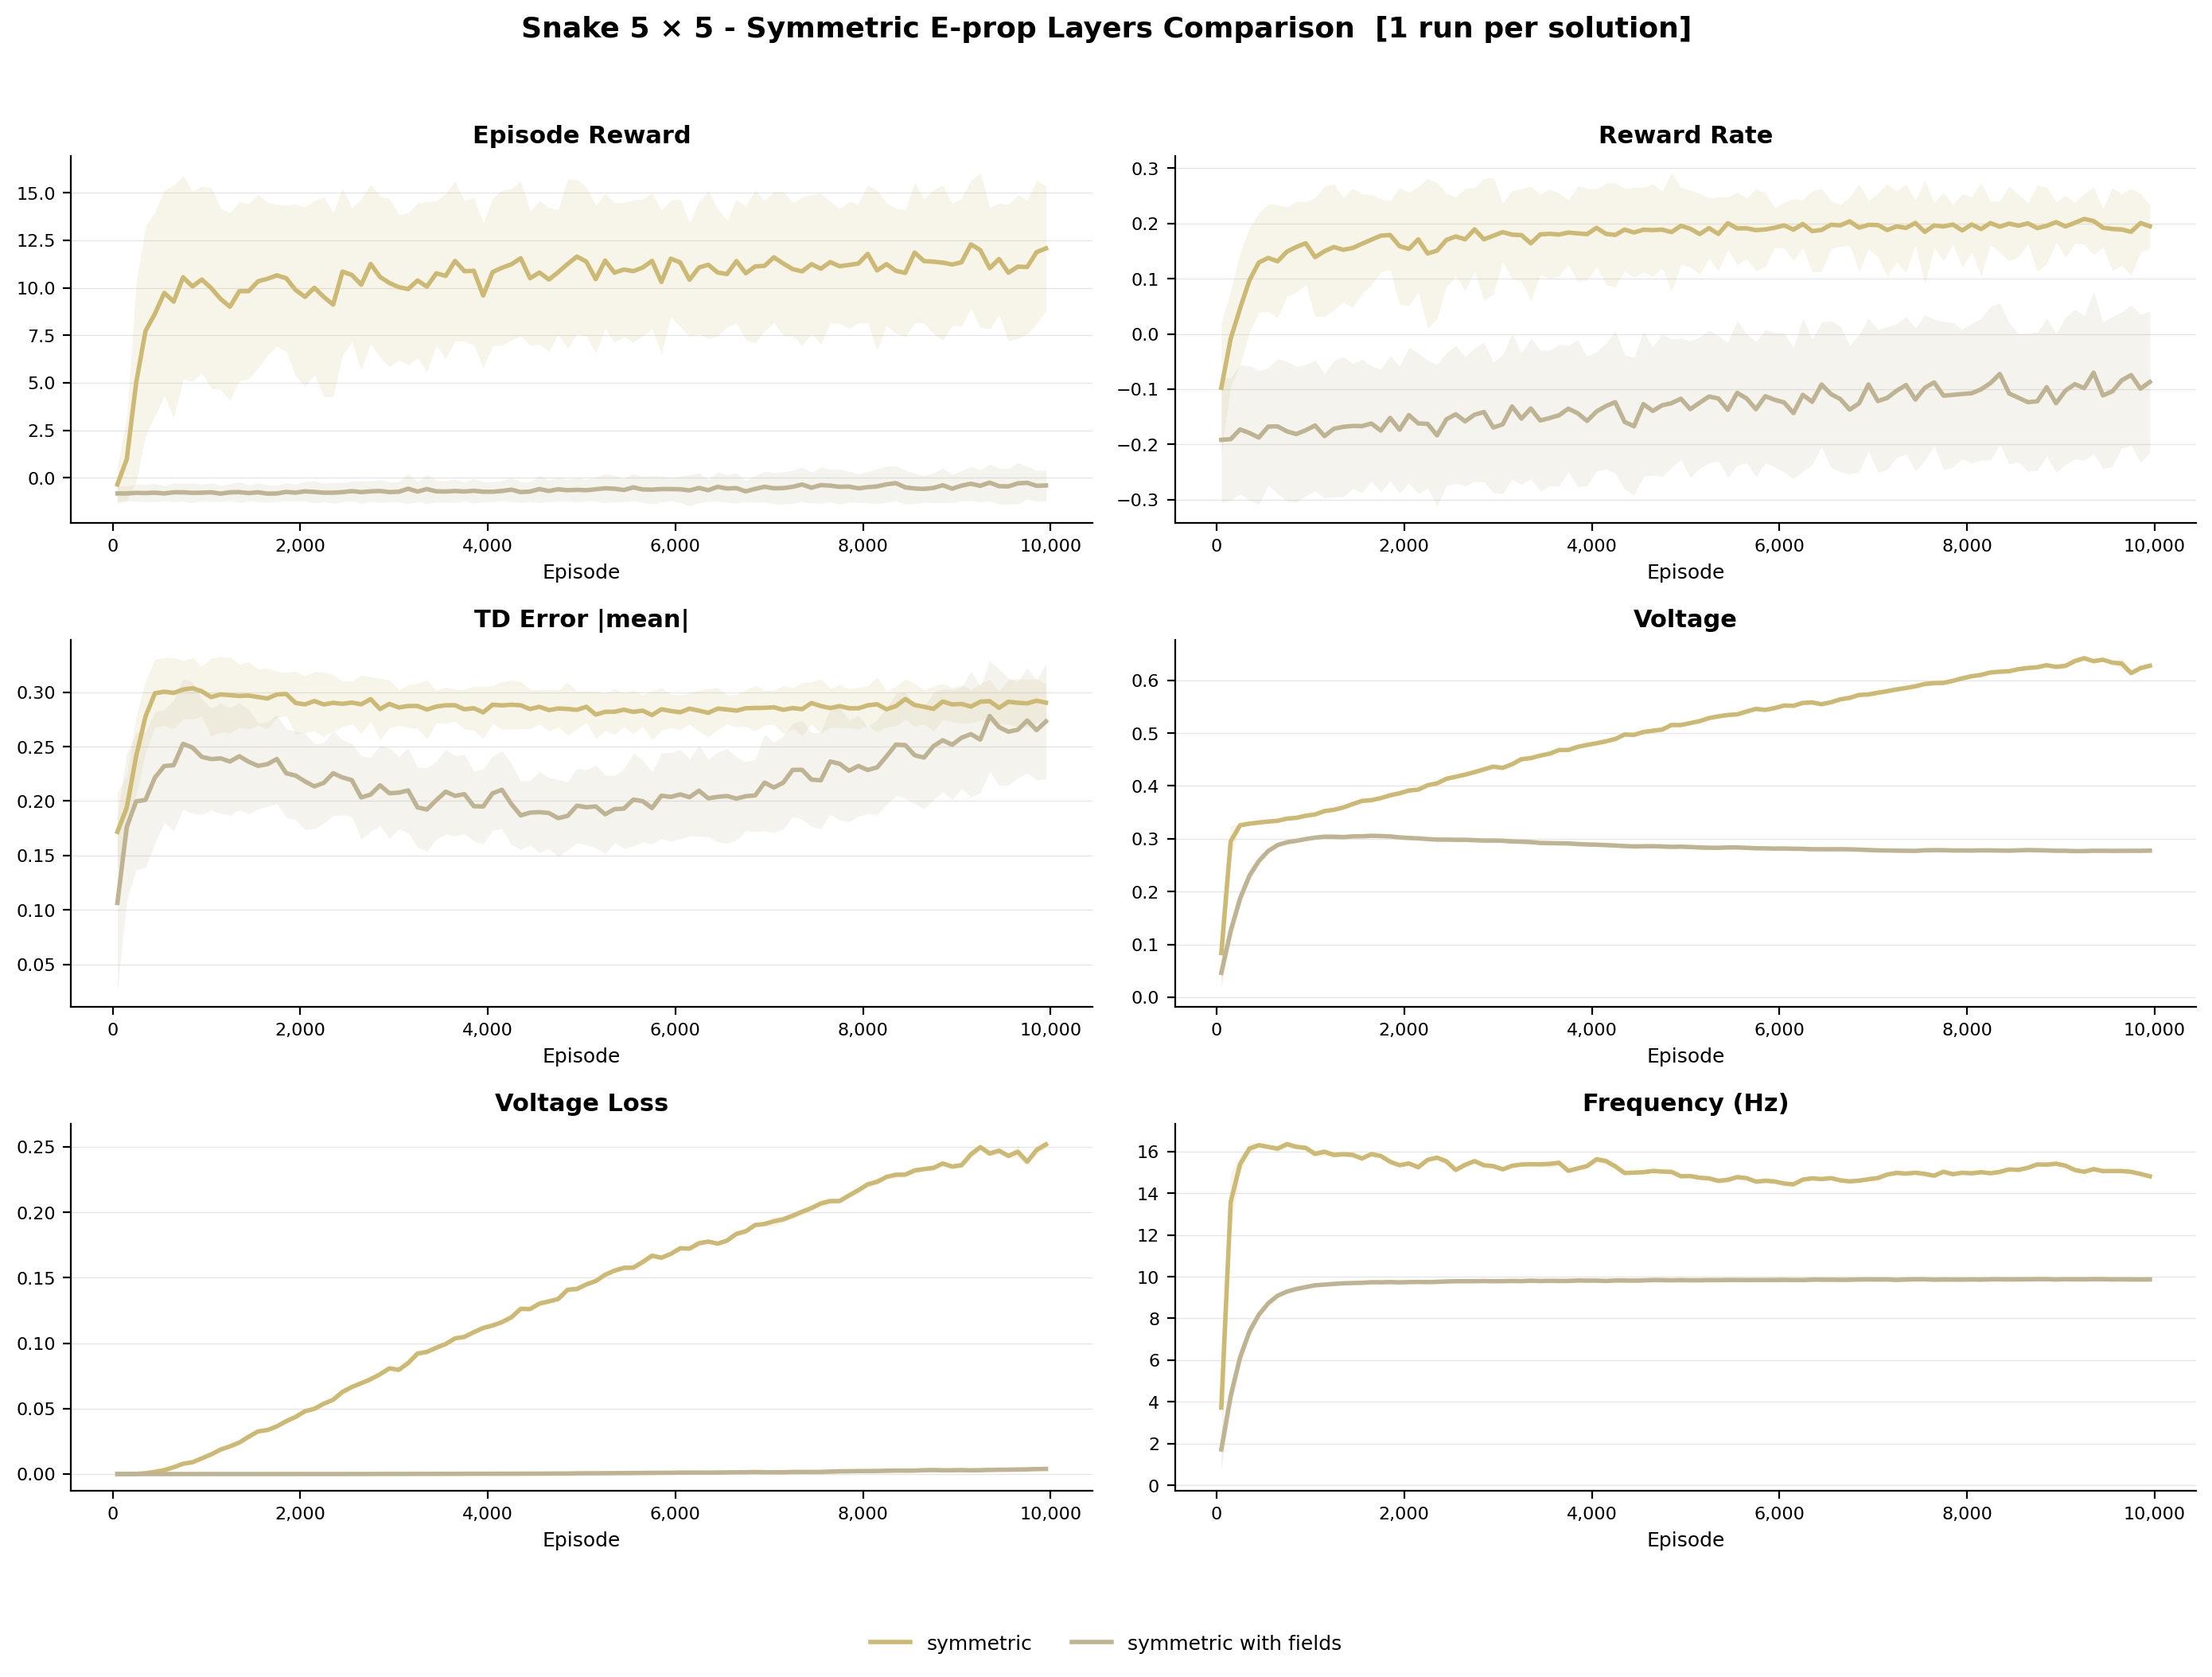
\includegraphics[width=0.5\linewidth]{images/SnakeSymmetric.png}
\caption{Symmetric e-prop on Snake $5\times5$, with and without the per-head
field layers (one run each). Six metrics over 10k episodes: episode reward,
reward rate, mean absolute TD error, voltage, voltage-regularisation loss, and
firing frequency. The plain variant attains the highest reward with the most
favourable dynamics; adding the field layers lengthens the causal path and
drives reward to near zero, because symmetric feedback is tied to the output
weights.
\pending{: to be regenerated.}}
\label{fig:symmetric}
\end{figure}

\subsection{\texorpdfstring{$\lambda$}{lambda}-Robustness Reverses Across Tasks}
\label{sec:results-lambda}

Several figures in this appendix include the \variant{combined} rule, which
sums the \variant{weight dist} update and the adaptive e-prop update for the
hidden weights. In practice it behaves much like \variant{weight dist}. A
plausible reason is an imbalance in the current setup rather than an
incompatibility between the two rules: the perturbation update receives a
dense TD signal at every timestep, whereas the policy part of adaptive
e-prop's learning signal only arrives at the action-sampling steps, every $K$
integration steps, so the sum is dominated by the dense term. Adding the
perturbation update from the start may also prevent the forward weights from
aligning with adaptive e-prop's feedback weights. A fair test of whether the
two families can work together would first let adaptive e-prop align its
feedback, then introduce the perturbation update, ideally with a
continuously-defined action head that removes the imbalance; we leave this to
future work.\pending{}

Neither rule is uniformly more robust to $\lambda$. On Snake, adaptive e-prop
tolerates almost the full range, failing only at $\lambda=0.99$, while the
perturbation-based variant shows a narrower, less monotonic band
(Fig.~\ref{fig:lambda-snake}). On Pac-Man the
ordering \emph{reverses}: the distributed variant learns promptly across
$\lambda\in\{0.4,0.5,0.6\}$ while adaptive e-prop shows an inconsistent, often
delayed onset (Fig.~\ref{fig:lambda-pacman}). This reversal is itself informative: robustness to the
credit-assignment horizon is not an intrinsic property of either algorithm but
depends on the task. Distributed e-prop also exhibits (at least) \emph{two}
distinct large-$\lambda$ failure modes (runaway high-frequency firing and,
separately, drift toward silence), so its robustness should not be
overstated.\pending{}

\begin{figure}[H]
\centering
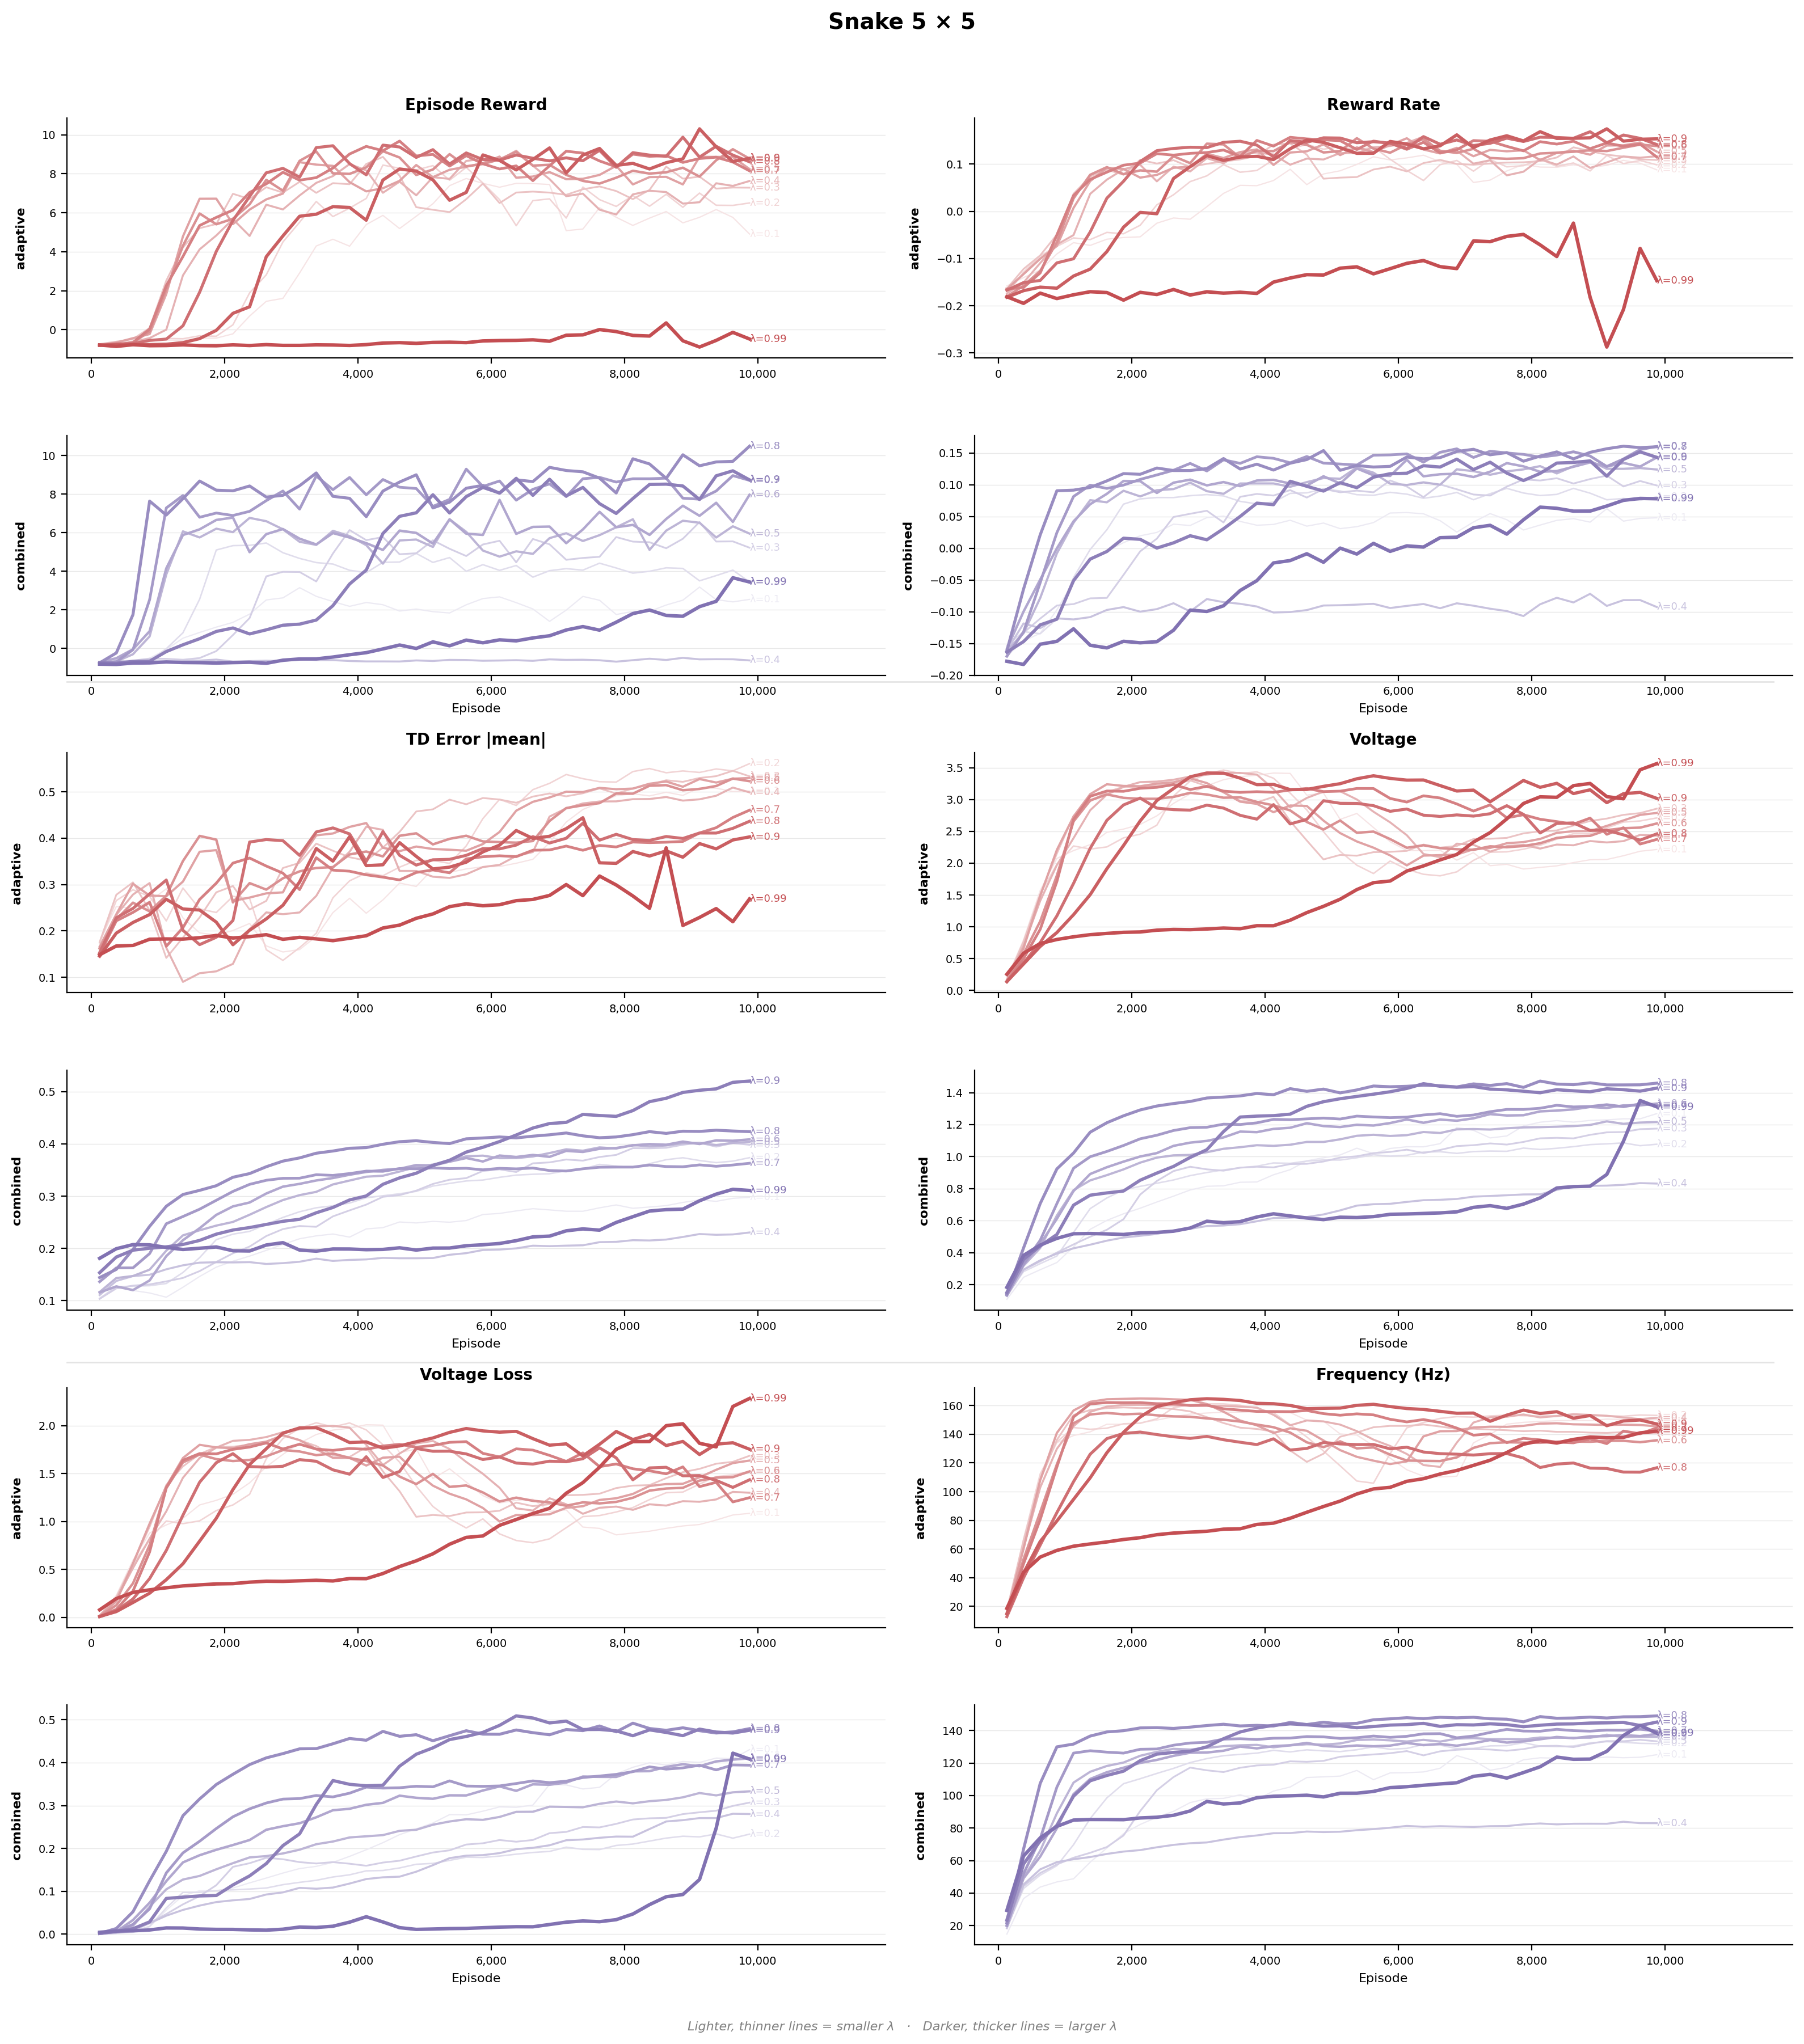
\includegraphics[width=\linewidth]{images/SnakeLambdaComparison.png}
\caption{$\lambda$ sweep on Snake $5\times5$ (10k episodes) for adaptive e-prop
(red) and \variant{combined} (purple); lighter/thinner lines are smaller $\lambda$.
Adaptive e-prop is robust across the range, failing only at $\lambda=0.99$; the
perturbation-based variant is less uniform.
\pending{: to be regenerated.}}
\label{fig:lambda-snake}
\end{figure}

\begin{figure}[H]
\centering
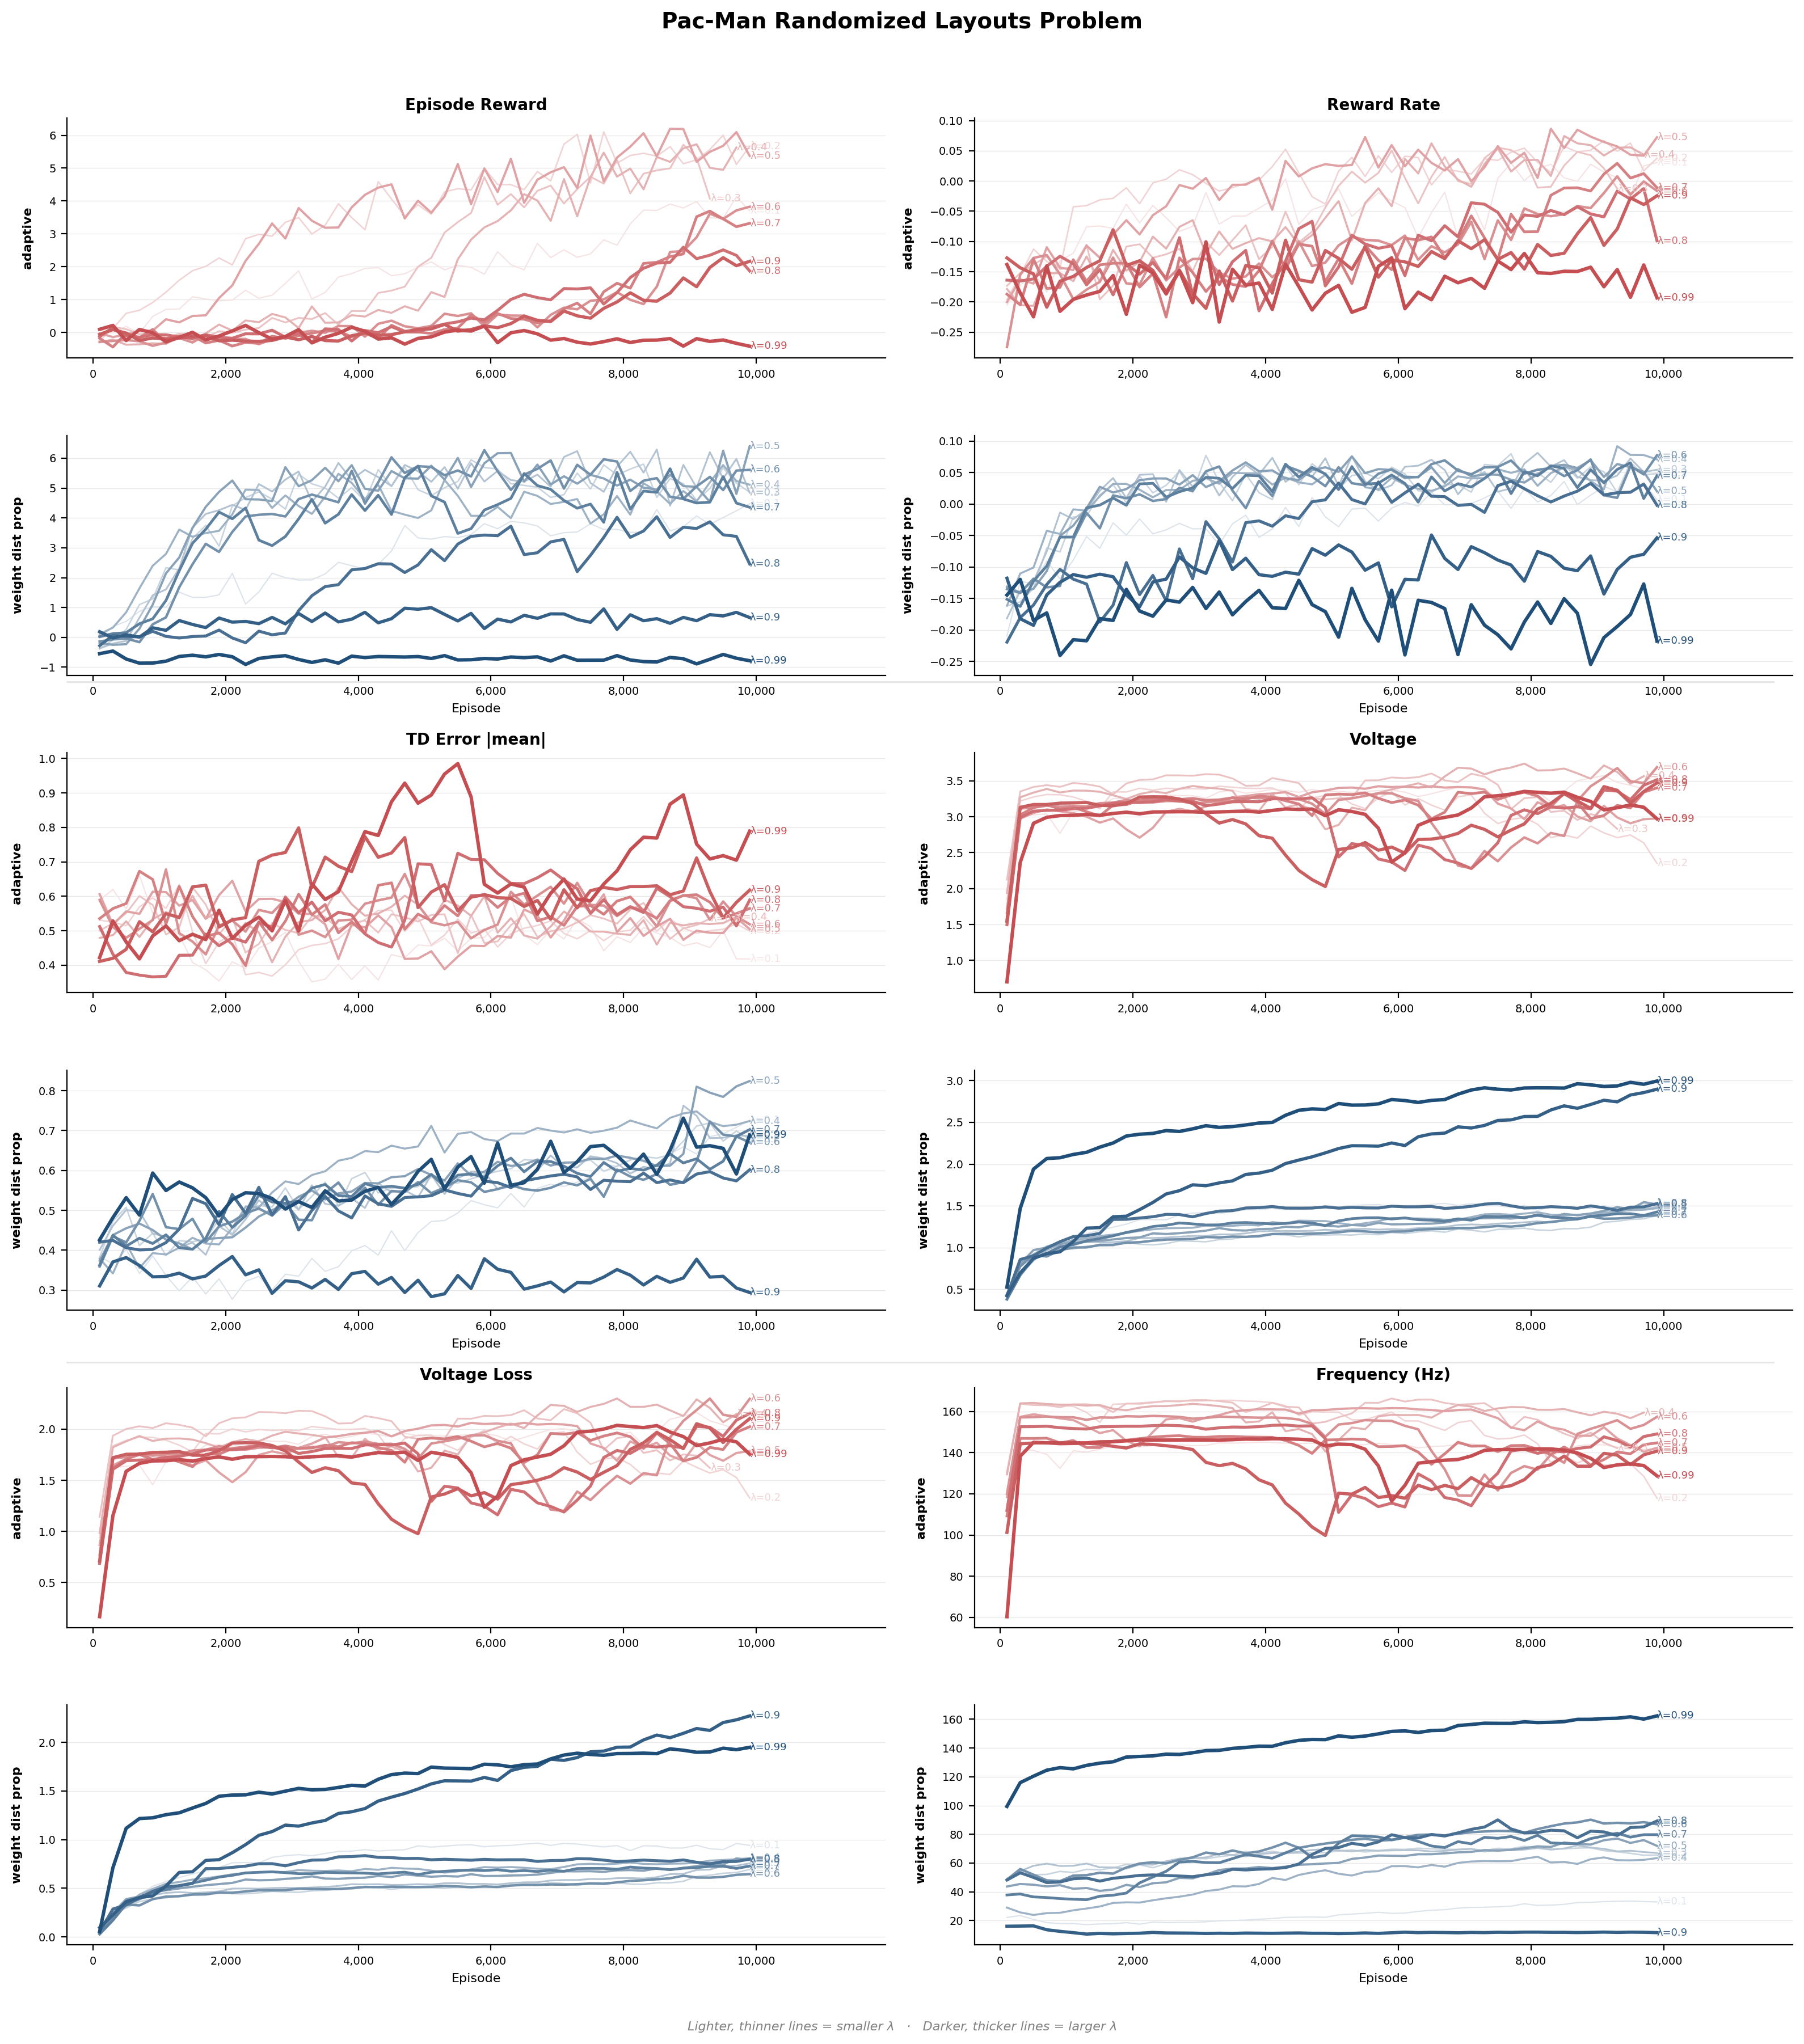
\includegraphics[width=\linewidth]{images/PacManComparisonLambdaGroups.png}
\caption{$\lambda$ sweep on the Pac-Man randomised-layouts problem for adaptive
e-prop (red) and \variant{weight dist prop} (blue). The ordering reverses relative
to Snake: the distributed variant learns promptly across a wide $\lambda$ range
while adaptive e-prop shows an inconsistent, often delayed onset. Large
$\lambda$ destabilises the distributed rule in two distinct directions
(runaway firing vs.\ silence).
\pending{: to be regenerated.}}
\label{fig:lambda-pacman}
\end{figure}

\subsection{Pac-Man: Standard Neuron Model}
\label{sec:results-pacman-unmodified}

On the Pac-Man randomised-layouts problem~\citep{denero2010pacman} (five
seeds), distributed variants reach higher episode rewards than adaptive
e-prop, converging to comparable reward rates, with more stable TD error,
voltage, and frequency (Fig.~\ref{fig:pacman}).\pending{}


\begin{figure}[H]
\centering
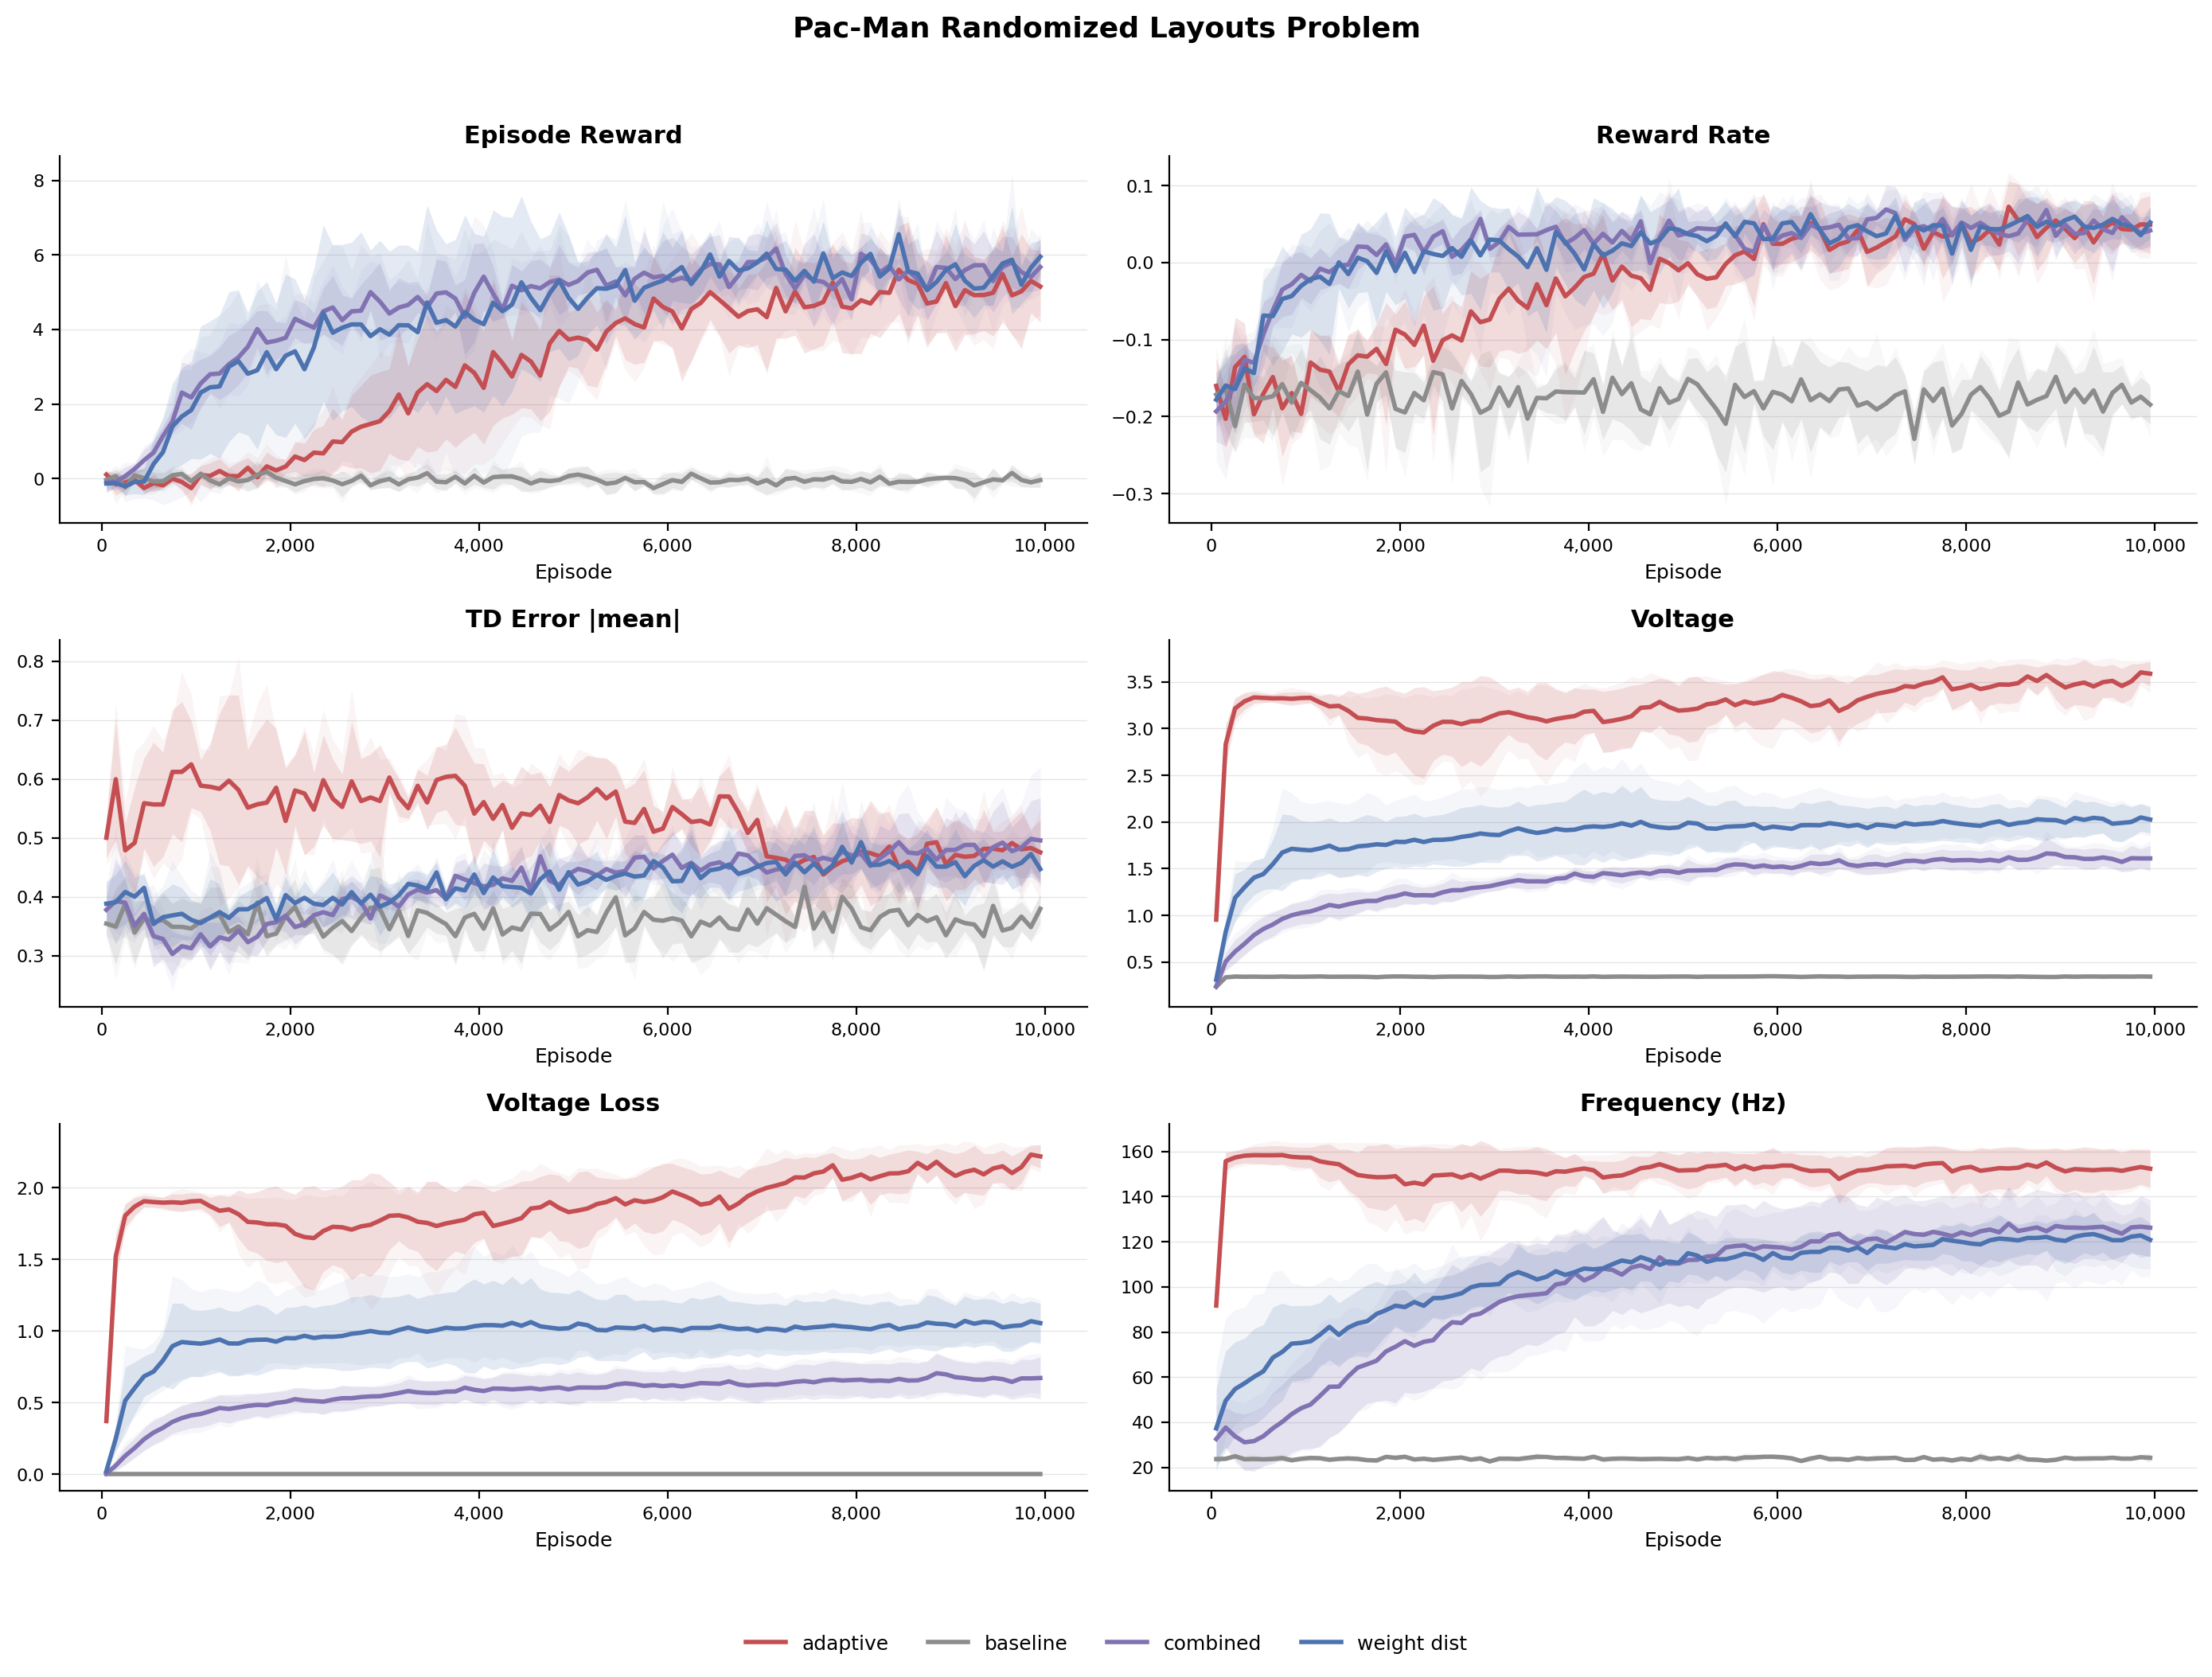
\includegraphics[width=\linewidth]{images/PacManComparison.png}
\caption{Distributed e-prop variants vs.\ adaptive e-prop on Pac-Man
randomised layouts (five seeds, shaded s.d.). Distributed variants reach higher
episode reward at comparable reward rate, with more stable TD error, voltage,
and frequency; \variant{combined} again tracks the distributed family.
\pending{: to be regenerated.}}
\label{fig:pacman}
\end{figure}

\subsection{Pac-Man: No Integration During the Refractory Period}
\label{sec:results-pacman-nidrp}

Under a neuron model that does not integrate inputs during the refractory
period, which violates an assumption of e-prop's analytical eligibility
derivation, adaptive e-prop barely learns and its dynamics diverge, while the
distributed variants, whose credit assignment rests on perturbation
correlations rather than on that derivation, learn with well-regulated spiking
(Fig.~\ref{fig:pacman-nidrp}).\pending{}

\begin{figure}[H]
\centering
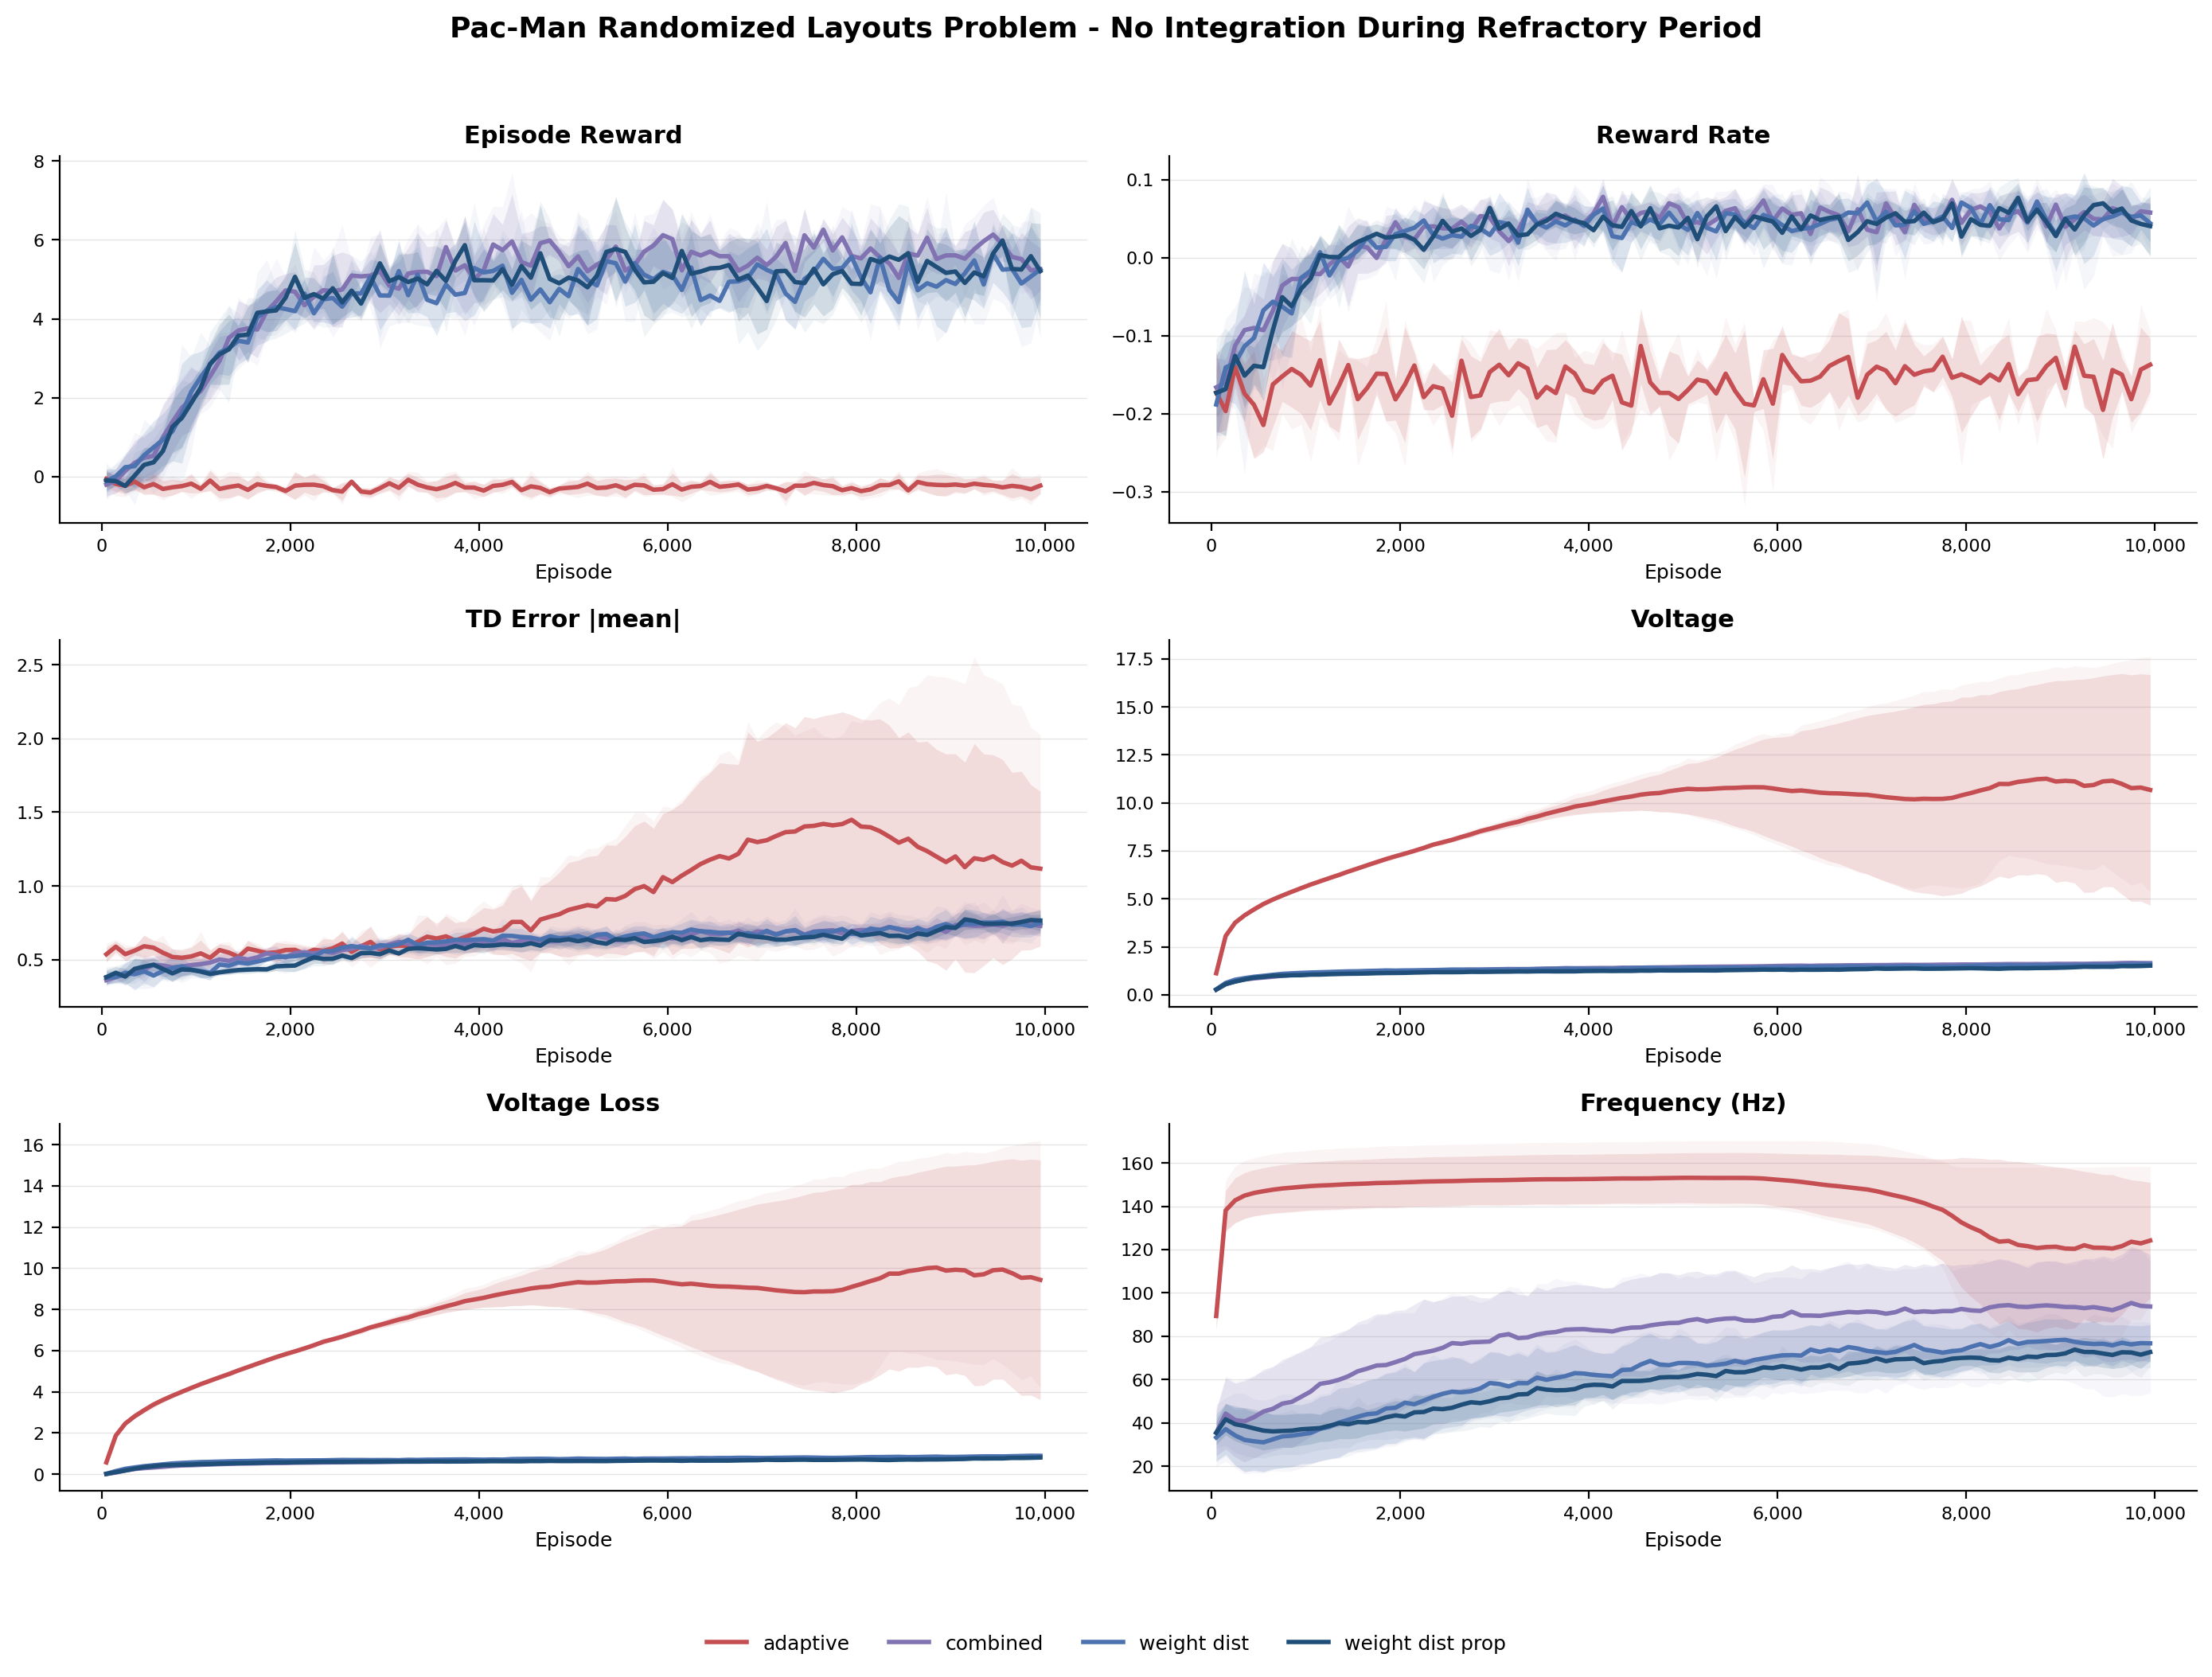
\includegraphics[width=\linewidth]{images/PacManComparisonNoIntegration.png}
\caption{Distributed e-prop variants vs.\ adaptive e-prop on Pac-Man
randomised layouts under the no-integration-during-refractory-period neuron
variant (five seeds, shaded s.d.). Adaptive e-prop barely learns and its
dynamics diverge, while the distributed variants learn successfully with
well-regulated spiking, evidence that perturbation-based credit assignment is
less sensitive to violations of e-prop's analytical assumptions.
\pending{: to be regenerated.}}
\label{fig:pacman-nidrp}
\end{figure}

\subsection{Structured Routing of the Perturbation Signal}
\label{app:routing}

\begin{figure}[H]
\centering
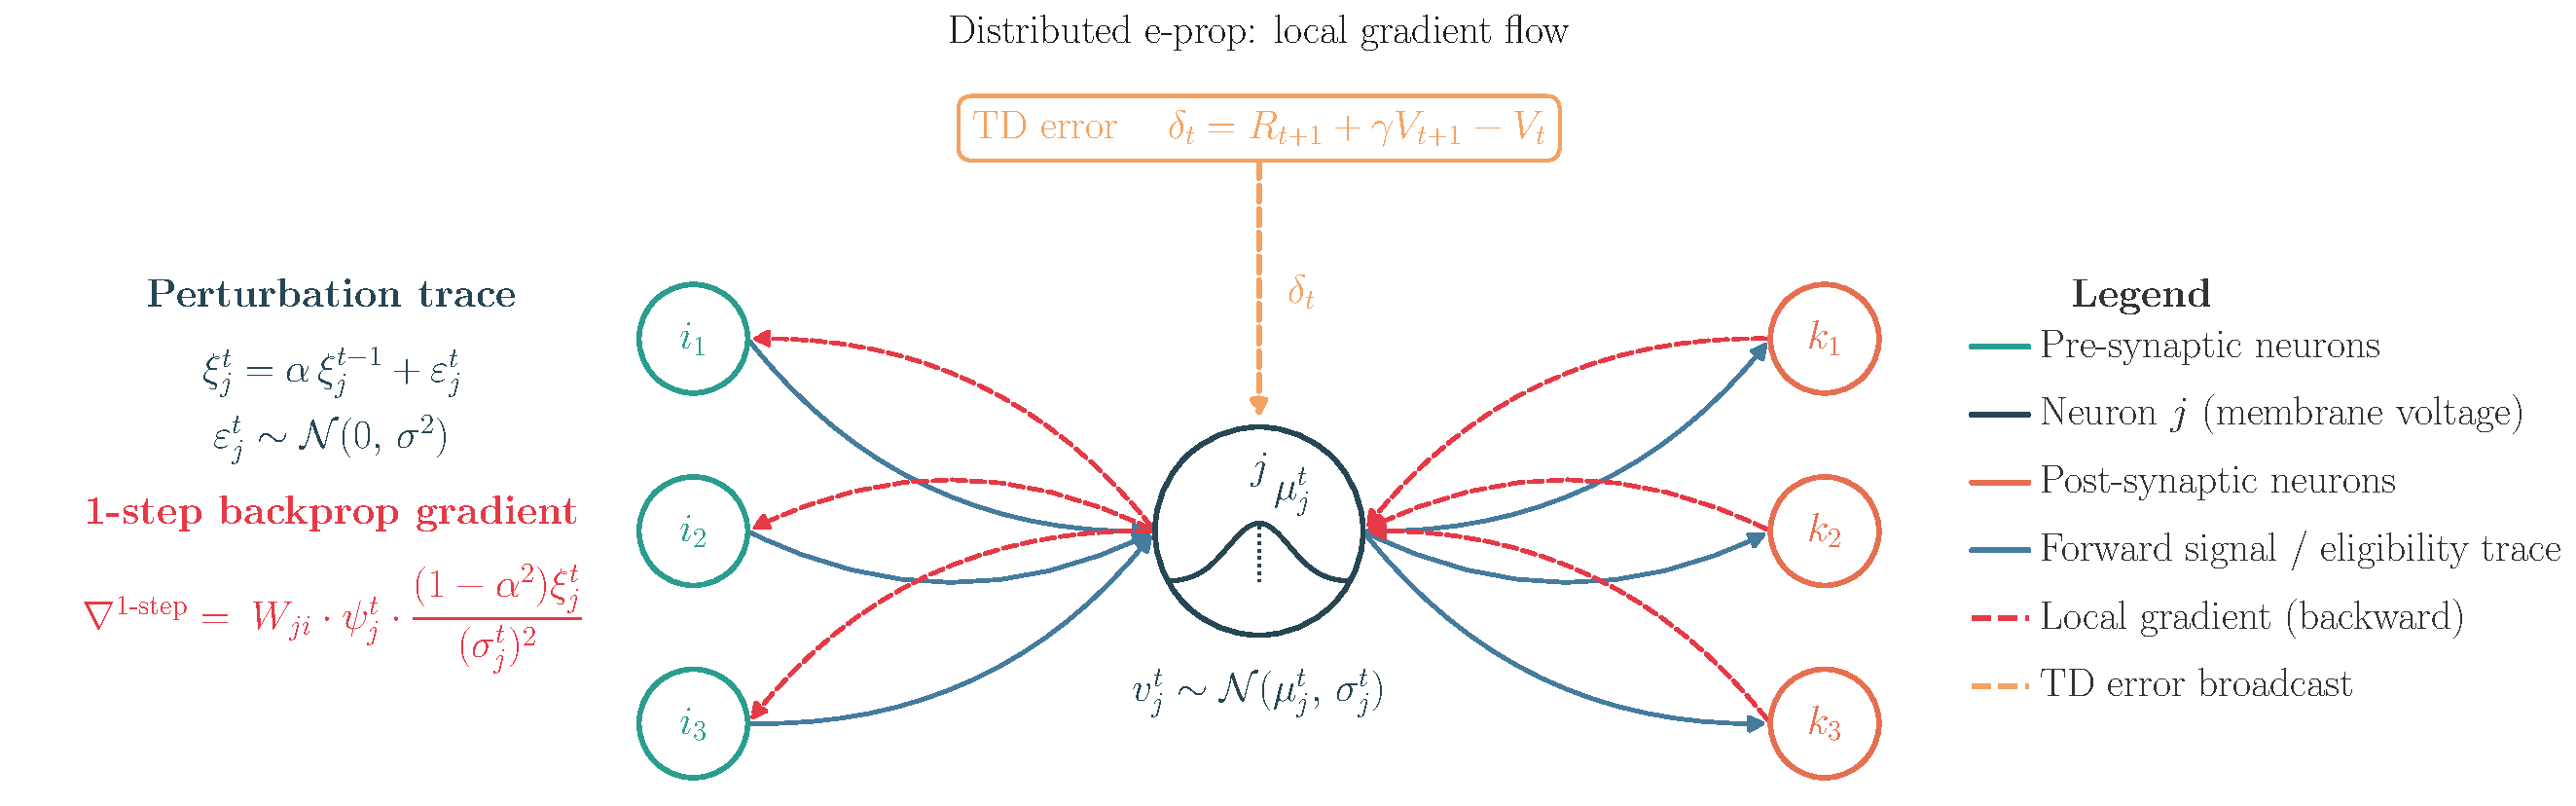
\includegraphics[width=0.95\linewidth]{images/distributed_eprop_diagram.pdf}
\caption{Local gradient flow in distributed e-prop. Neuron $j$ holds a
stochastic membrane $v^t_j\sim\mathcal{N}(\mu^t_j,\sigma^t_j)$; its perturbation
trace $\xi^t_j=\alpha\xi^{t-1}_j+\varepsilon^t_j$ accumulates exploration along
each incoming synapse. Spikes propagate forward; a single global TD error
$\delta_t$ is broadcast from the critic. In routed variants the local signal is
sent back through the recurrent weights themselves.}
\label{fig:schematic}
\end{figure}

Section~\ref{sec:distributed} notes that each neuron's local policy-gradient
estimator, $g^t_j=(1-\alpha^2)\xi^t_j\psi^t_j/\sigma_j^2$, can be propagated
through the recurrent weights themselves, $L^t_j=\sum_k W_{kj}\,g^t_k$,
reusing symmetric-e-prop machinery with the recurrent connectivity. We tried
two ways of folding this routed signal into the hidden-weight update. The
first adds it to the local term as a separate contribution,
\begin{equation}
p^{\,t}_{ji} = \lambda\, p^{\,t-1}_{ji} + e^t_{ji}\left(g^t_j + L^t_j\right),
\qquad \Delta W_{ji} = -\eta\sum_t \delta_t\, p^{\,t}_{ji},
\label{eq:routed-update}
\end{equation}
which sits between the broadcast-only rule of
Eq.~\eqref{eq:distributed-update} ($L^t_j=0$) and a fully routed rule. The
second multiplies the local term by $(1+L^t_j)$: $e^t_{ji}\,g^t_j(1+L^t_j)$
expands to $e^t_{ji}\,g^t_j + e^t_{ji}\,g^t_j\,L^t_j$, so the $1$ recovers
Eq.~\eqref{eq:distributed-update} unchanged and the routed signal adds a
multiplicative interaction term on top of it, on the reasoning that a
neuron's own perturbation should count for more when the recurrent network
also implicates it. Neither addition
improved on the broadcast-only rule in our experiments
(Section~\ref{sec:results}), and the multiplicative term made the rule
harder to reason about without a compensating benefit, so we do not use
either in the main text.\pending{: ablation figures for both routed variants
to be added.}

\section{Hyperparameters}
\label{app:hyper}
Table~\ref{tab:hyper} lists the settings shared by every experiment and
Table~\ref{tab:hyper-task} those that vary by task or rule. Discount and trace
decays are given per environment step; per-timestep values follow by raising to
the $1/K$ power.
\todo{Fill the red cells in Table~\ref{tab:hyper-task} from the final run
configs (ideally generated by a script from the config files). Check the
per-task $\lambda$ against Section~\ref{sec:tdlambda}, which currently says
$\lambda=0.8$ throughout. Move any row that turns out identical across tasks to
Table~\ref{tab:hyper}.}

\begin{table}[h]
\centering\footnotesize
\begin{tabular}{@{}lll@{}}
\toprule
\textbf{Group} & \textbf{Symbol / name} & \textbf{Value} \\
\midrule
\multicolumn{3}{@{}l}{\textit{Neuron (ALIF, all hidden populations)}} \\
& threshold $v_{\mathrm{th}}$ & $0.61$ \\
& membrane $\tau_{\mathrm{mem}}$ & $10$\,ms \\
& refractory $\tau_{\mathrm{refrac}}$ & $3$\,ms \\
& adaptation $\tau_{\mathrm{adapt}}$ & $300$\,ms \\
& adaptation strength $\beta$ & $0.0174$ \\
& surrogate sharpness $\gamma_{\mathrm{pd}}$ & $0.3$ \\
\midrule
\multicolumn{3}{@{}l}{\textit{Architecture}} \\
& hidden E & $20\times20\times3$ ($1200$) \\
& hidden I / field & $15\times15\times3$ ($675$) \\
& value head & $1$ \\
\midrule
\multicolumn{3}{@{}l}{\textit{Connectivity}} \\
& profile & toroidal Gaussian \\
& $\sigma_{\mathrm{in}}$ / $\sigma_{\mathrm{h}}$ & $0.1$ / $0.05$ \\
& target fan-in $K_{\mathrm{in}}$ & $100$ \\
\midrule
\multicolumn{3}{@{}l}{\textit{Learning}} \\
& optimiser (distributed) & AdaBelief ($\beta_1=0.99$, $\beta_2=0.99999$) \\
& optimiser (adaptive, symmetric) & Adam ($\beta_1=0.9$, $\beta_2=0.999$) \\
& batch size / update schedule & $1$ / every simulation timestep \\
& action window $K$ & $30$ steps \\
& discount $\gamma$ (per env.\ step) & $0.5$ \\
& firing-rate reg.\ $c_{\mathrm{reg}}$ & $10^{-4}$ \\
& target rate $F^{*}$ & $10$\,Hz \\
& target rate $F^{*}$ (baseline) & $120$\,Hz \\
& L2 Init strength $c_{\mathrm{init}}$ & $10^{-5}$ \\
\bottomrule
\end{tabular}
\caption{Hyperparameters shared by every experiment.
\pending{: appendix results (Appendix~\ref{app:extra-results}) were produced
with plain Adam and without L2 Init.}}
\label{tab:hyper}
\end{table}

\begin{table}[h]
\centering\footnotesize
\begin{tabular}{@{}llccc@{}}
\toprule
\textbf{Group} & \textbf{Symbol / name} & \textbf{Snake} & \textbf{Pac-Man} & \textbf{Tic-Tac-Toe} \\
\midrule
\multicolumn{5}{@{}l}{\textit{Task and architecture}} \\
& policy head (actions) & $4$ & \tbd & \tbd \\
& input grid & \tbd & \tbd & \tbd \\
& field layers & yes & \tbd & \tbd \\
& training length & 20k episodes & \tbd & \tbd \\
\midrule
\multicolumn{5}{@{}l}{\textit{Learning}} \\
& trace decay $\lambda$ (per env.\ step) & $0.8$ & \tbd & \tbd \\
& learning rate $\eta$ (distributed) & \tbd & \tbd & \tbd \\
& learning rate $\eta$ (adaptive) & \tbd & \tbd & \tbd \\
& critic learning rate $\eta_V$ & \tbd & \tbd & \tbd \\
\midrule
\multicolumn{5}{@{}l}{\textit{Distributed perturbation}} \\
& $\log\sigma_j$ (neuron variant) & $-4.61$ & \tbd & \tbd \\
& $\log\sigma_{ji}$ (weight variants) & $-5$ & \tbd & \tbd \\
\bottomrule
\end{tabular}
\caption{Hyperparameters that vary by task or rule. \textcolor{red}{\textbf{?}}
marks values still to be filled in.}
\label{tab:hyper-task}
\end{table}


\end{document}